\documentclass[12pt,a4paper]{article}

% ---------- Codifica e lingua ----------
\usepackage{cmap}        % Rende il PDF ricercabile e il testo selezionabile
\usepackage[T1]{fontenc} % Codifica corretta (essenziale per l'italiano e gli accenti)
\usepackage[utf8]{inputenc}
\usepackage[italian,provide=*]{babel}

% ---------- Layout ----------
\usepackage[a4paper,top=2.6cm,bottom=2.6cm,left=2.6cm,right=2.6cm]{geometry}
\usepackage{graphicx}
\graphicspath{{img/}}
\usepackage{float}
\usepackage{booktabs}
\usepackage{caption}
\captionsetup{font=small,labelfont=bf,width=0.92\textwidth}
\usepackage{amsmath,amssymb}
\usepackage{xcolor}
\definecolor{bicoccablue}{RGB}{0,70,127}
\definecolor{boxgray}{RGB}{245,247,250}

% ---------- Intestazioni e titoli ----------
\usepackage{fancyhdr}
% Intestazioni di sezione colorate senza titlesec (non disponibile): redefinizione standard
\makeatletter
\renewcommand\section{\@startsection{section}{1}{\z@}%
  {-3.5ex \@plus -1ex \@minus -.2ex}{2.3ex \@plus.2ex}%
  {\normalfont\Large\bfseries}}
\renewcommand\subsection{\@startsection{subsection}{2}{\z@}%
  {-3.25ex\@plus -1ex \@minus -.2ex}{1.5ex \@plus .2ex}%
  {\normalfont\large\bfseries}}
\makeatother
\pagestyle{plain}

\usepackage[hidelinks]{hyperref}

\begin{document}

% ============================================================
% FRONTESPIZIO
% ============================================================
\begin{titlepage}
\centering
\vspace*{0.6cm}
{\Large\bfseries UNIVERSIT\`A DEGLI STUDI DI MILANO - BICOCCA\par}
\vspace{0.4cm}
{\large Dipartimento di Informatica, Sistemistica e Comunicazione (DISCo)\par}
\vspace{0.2cm}
{\large Corso di laurea in Data Science\par}
\vspace{1.2cm}

\rule{\textwidth}{0.4pt}\\[0.4cm]
{\LARGE\bfseries Studio di robustezza dei modelli di\\ machine learning al rumore nei dati\par}
\vspace{0.35cm}
{\large Progetto di \textit{Architetture Dati}\par}
\vspace{0.25cm}
{\normalsize Un'analisi sperimentale sul dataset MAGIC Gamma Telescope\par}
\rule{\textwidth}{0.4pt}\\[1.4cm]

\begin{minipage}{0.9\textwidth}
\centering
{\large\bfseries Autori\par}
\vspace{0.3cm}
{\large
Daniele Maccagnan \quad--\quad matricola [matricola]\\[0.25cm]
Matias Bonoli \quad--\quad matricola [matricola]\\[0.25cm]
Ashley Chudory \quad--\quad matricola [matricola]\\
}
\end{minipage}

\vfill
{\large Anno accademico 2025/2026\par}
\end{titlepage}

% ============================================================
% INDICE
% ============================================================
\tableofcontents
\thispagestyle{plain}
\clearpage

% ============================================================
% 1. INTRODUZIONE
% ============================================================
\section{Introduzione}\label{sec:intro}

In applicazioni reali la presenza di imperfezioni nei dati come
misurazioni imprecise, errori di annotazione, valori mancanti e anomalie,
rappresenta la norma. L'obiettivo di questa analisi non è identificare il 
modello in grado di raggiungere l'accuratezza massima sui dati ideali, bensì 
quantificare la resistenza di ciascun modello al progressivo degrado delle 
informazioni. A tale scopo, viene misurata la robustezza di tre modelli 
supervisionati corrompendo il training set in modo controllato, attraverso 
sette diverse tipologie di rumore.

L'obiettivo dello studio non è decretare un singolo modello vincente, ma
comprendere come e perché le prestazioni peggiorino in base al tipo di
disturbo introdotto nei dati. La procedura prevede inizialmente il
calcolo di una baseline sui dati integri. Successivamente,
i modelli vengono riaddestrati su versioni del training set
alterate con tre livelli di intensità crescente: 10\%, 25\% e 40\%.
Per garantire la correttezza della valutazione, le metriche vengono
sempre calcolate su un test set mantenuto pulito e inalterato.

I tre modelli analizzati sono una rete neurale classica,
una sua variante dotata di meccanismi di regolarizzazione
e un Random Forest. I sette disturbi introdotti agiscono
direttamente su feature, etichette, valori mancanti,
outlier e sulla disponibilità stessa delle variabili. Infine,
viene affiancato un esperimento non supervisionato tramite K-Means,
svolto per osservare l'impatto del rumore quando il modello lavora
senza avere accesso alle etichette.

Per garantire la completa riproducibilità degli esperimenti, è stato fissato un 
seme casuale globale (\texttt{seed = 42}) su tutte le componenti stocastiche, 
comprendendo lo split dei dati, l'inizializzazione dei pesi delle reti, 
l'iniezione del rumore e i processi di campionamento del Random Forest e del 
K-Means.

% ============================================================
% 2. DATASET
% ============================================================
\section{Il dataset}\label{sec:dataset}

Il dataset utilizzato è il MAGIC Gamma Telescope, generato tramite simulazioni 
Monte Carlo del telescopio Cherenkov MAGIC. Ogni osservazione descrive la 
traccia luminosa, di forma approssimativamente ellittica, lasciata da un 
evento atmosferico sul piano del rivelatore. Il task consiste in una 
classificazione binaria con un preciso significato fisico: distinguere i 
segnali utili, prodotti da raggi gamma, dal rumore di fondo generato da adroni. 

Il dataset originario comprende $19\,020$ osservazioni e $11$ attributi: dieci 
feature continue e una variabile target. Le feature codificano la geometria e 
la distribuzione di intensità dell'immagine. In fase 
di preparazione, è stata effettuata una mappatura numerica delle due classi: 
\texttt{h}~$\rightarrow 0$ per gli adroni e \texttt{g}~$\rightarrow 1$ 
per i gamma. La Tabella~\ref{tab:feature} riporta la descrizione 
dettagliata delle feature.

\begin{table}[H]\centering\small
\caption{Le dieci feature continue del dataset MAGIC e il loro significato.}\label{tab:feature}
\begin{tabular}{ll}
\toprule
\textbf{Feature} & \textbf{Descrizione} \\
\midrule
\texttt{fLength}   & lunghezza dell'asse maggiore dell'ellisse dell'immagine \\
\texttt{fWidth}    & lunghezza dell'asse minore dell'ellisse \\
\texttt{fSize}     & logaritmo della somma delle intensità di tutti i pixel \\
\texttt{fConc}     & rapporto di concentrazione dei due pixel più intensi \\
\texttt{fConc1}    & rapporto di concentrazione del pixel più intenso \\
\texttt{fAsym}     & asimmetria della distribuzione lungo l'asse maggiore \\
\texttt{fM3Long}   & momento terzo (asimmetria) lungo l'asse maggiore \\
\texttt{fM3Trans}  & momento terzo lungo l'asse minore \\
\texttt{fAlpha}    & angolo tra l'asse maggiore e la direzione del centro del campo \\
\texttt{fDist}     & distanza dal centro del campo all'origine dell'ellisse \\
\midrule
\texttt{class}     & target: $1$ = gamma (segnale), $0$ = adrone (fondo) \\
\bottomrule
\end{tabular}
\end{table}

% ============================================================
% 3. SUDDIVISIONE DEI DATI
% ============================================================
\section{Suddivisione in training, validation e test}\label{sec:split}

Il dataset è stato suddiviso in tre partizioni prima di procedere a qualsiasi 
altra operazione, inclusa l'analisi esplorativa. Questa separazione preventiva 
è fondamentale per evitare che le statistiche calcolate sull'intero campione 
possano influenzare le scelte modellistiche, causando \textit{data leakage}. 
Limitando l'analisi esplorativa e il calcolo dei parametri di preprocessing al 
solo training set, validation e test set si mantengono come stime rigorose e 
imparziali della capacità di generalizzazione.

Lo split è stato eseguito seguendo le proporzioni $60\%$ / $20\%$ / $20\%$ 
rispettivamente per training, validation e test. La suddivisione è stratificata 
rispetto alla variabile target: ogni sottoinsieme preserva la medesima 
proporzione tra gamma e adroni presente nel dataset originale. Questa 
accortezza si rende necessaria a causa dello sbilanciamento delle classi; 
un campionamento puramente casuale rischierebbe di produrre insiemi con una 
rappresentanza insufficiente della classe minoritaria. Si ottengono così 
$11\,412$ campioni di training, $3\,804$ di validation e $3\,804$ di test. Il 
validation set viene utilizzato per monitorare l'addestramento, mentre il test 
set rimane isolato per la valutazione finale.

% ============================================================
% 4. EDA
% ============================================================
\section{Analisi esplorativa dei dati}\label{sec:eda}

L'analisi esplorativa viene condotta esclusivamente sul training set per
garantire il corretto isolamento delle altre partizioni. Il dataset originale
non presenta valori nulli, fornendo una base di partenza integra; in questo
modo lo studio rimane rigorosamente controllato, poiché ogni successiva
corruzione viene introdotta in maniera deliberata e quantificabile. In fase
esplorativa sono stati inoltre individuati $41$ record duplicati nel training
set: data la loro incidenza trascurabile (circa lo $0{,}4\%$ dei campioni),
essi vengono rimossi unicamente ai fini delle statistiche e dei grafici
descrittivi presentati in questa sezione, portando il conteggio da $11\,412$ a
$11\,371$ osservazioni; l'addestramento dei modelli viene invece condotto
sull'intero training set, dato che l'effetto numerico dei duplicati sulle
metriche finali è in ogni caso irrilevante.

La Figura~\ref{fig:pie} illustra la distribuzione della variabile target, 
evidenziando un netto sbilanciamento. La classe gamma costituisce 
il $64{,}8\%$ delle osservazioni, mentre gli adroni rappresentano il restante 
$35{,}2\%$, configurando un rapporto di quasi due a uno. Questo squilibrio 
fissa una linea di base operativa: un classificatore \textit{dummy} che 
prevedesse sistematicamente la classe maggioritaria otterrebbe un'accuratezza 
prossima al $65\%$. Di conseguenza, qualsiasi modello predittivo deve 
necessariamente superare questa soglia per dimostrare un effettivo apprendimento.

\begin{figure}[H]\centering
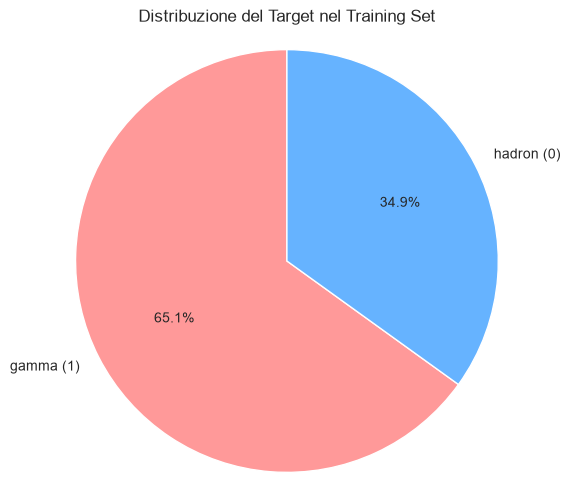
\includegraphics[width=0.55\textwidth]{eda_pie}
\caption{Distribuzione delle due classi nel training set: i gamma (segnale) sono quasi il doppio degli adroni (fondo).}
\label{fig:pie}
\end{figure}

Le distribuzioni delle variabili continue (Figura~\ref{fig:hist}) risultano 
prevalentemente asimmetriche (\textit{right-skewed}), con densità concentrate 
sui valori inferiori e lunghe code verso destra. Questa marcata asimmetria 
rende la mediana uno stimatore di tendenza centrale più robusto alle code
rispetto alla media, pur senza garantire \textit{a priori} un'imputazione
empiricamente migliore. Si osserva inoltre una notevole 
eterogeneità nelle scale numeriche, che spaziano da unità singole a centinaia, 
rendendo necessaria una successiva normalizzazione.

\begin{figure}[H]\centering
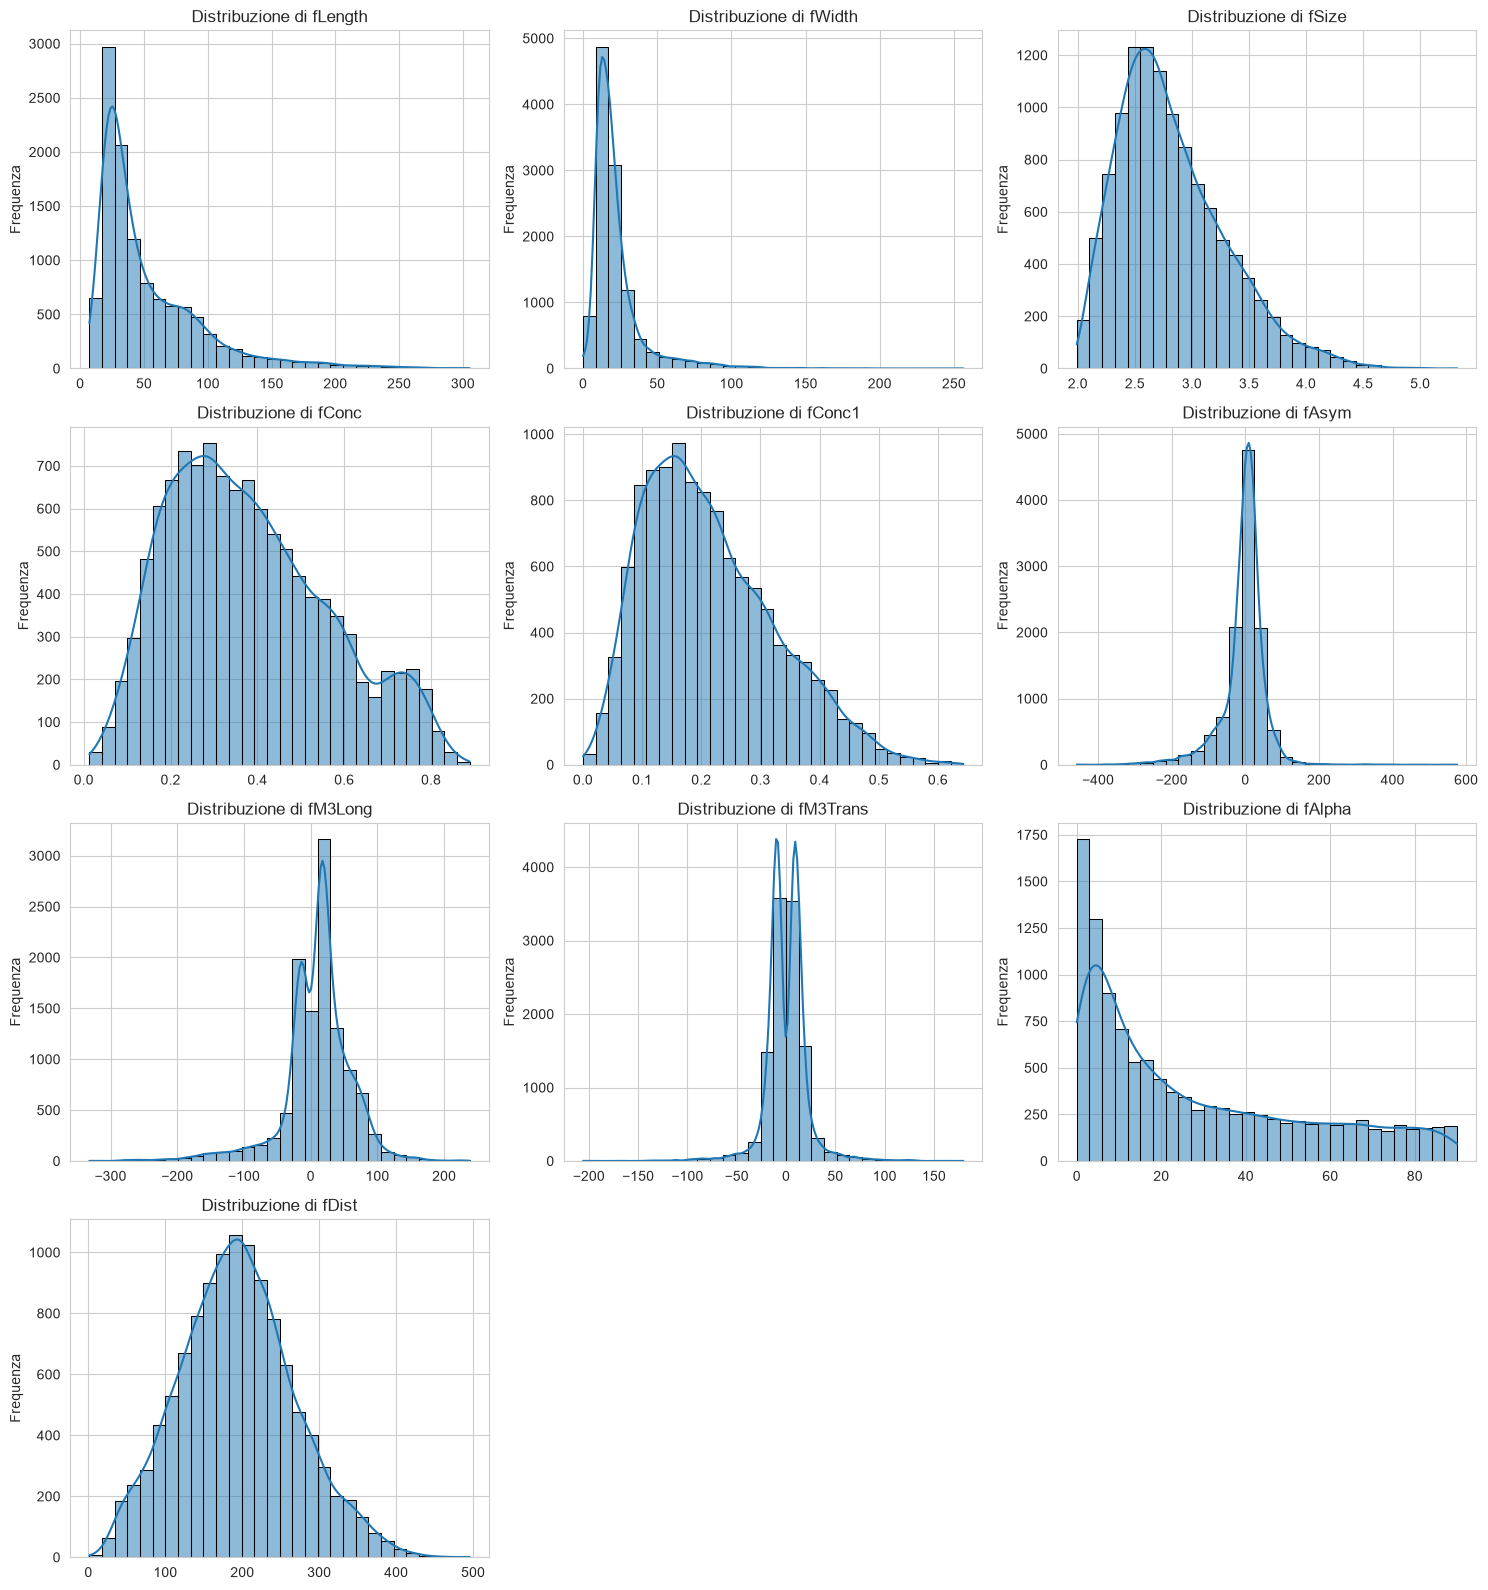
\includegraphics[width=0.95\textwidth]{eda_hist}
\caption{Istogrammi delle dieci feature continue (training set): distribuzioni asimmetriche, con code lunghe e scale eterogenee.}
\label{fig:hist}
\end{figure}

I boxplot suddivisi per classe (Figura~\ref{fig:box}) permettono di valutare il 
potere discriminante intrinseco delle singole feature. La variabile 
\texttt{fAlpha} mostra la capacità di separazione più netta: i valori associati 
ai gamma si concentrano in un range ristretto e basso, mentre quelli degli adroni 
presentano un'elevata dispersione. Seguono \texttt{fLength}, \texttt{fWidth} e 
\texttt{fSize}, che offrono un buon contributo informativo. Al contrario, feature 
come \texttt{fM3Trans} e \texttt{fAsym} esibiscono distribuzioni ampiamente 
sovrapposte tra le due classi, fornendo un apporto discriminante marginale. 
L'informazione utile alla classificazione risulta pertanto concentrata in un 
sottoinsieme limitato di variabili.

\begin{figure}[H]\centering
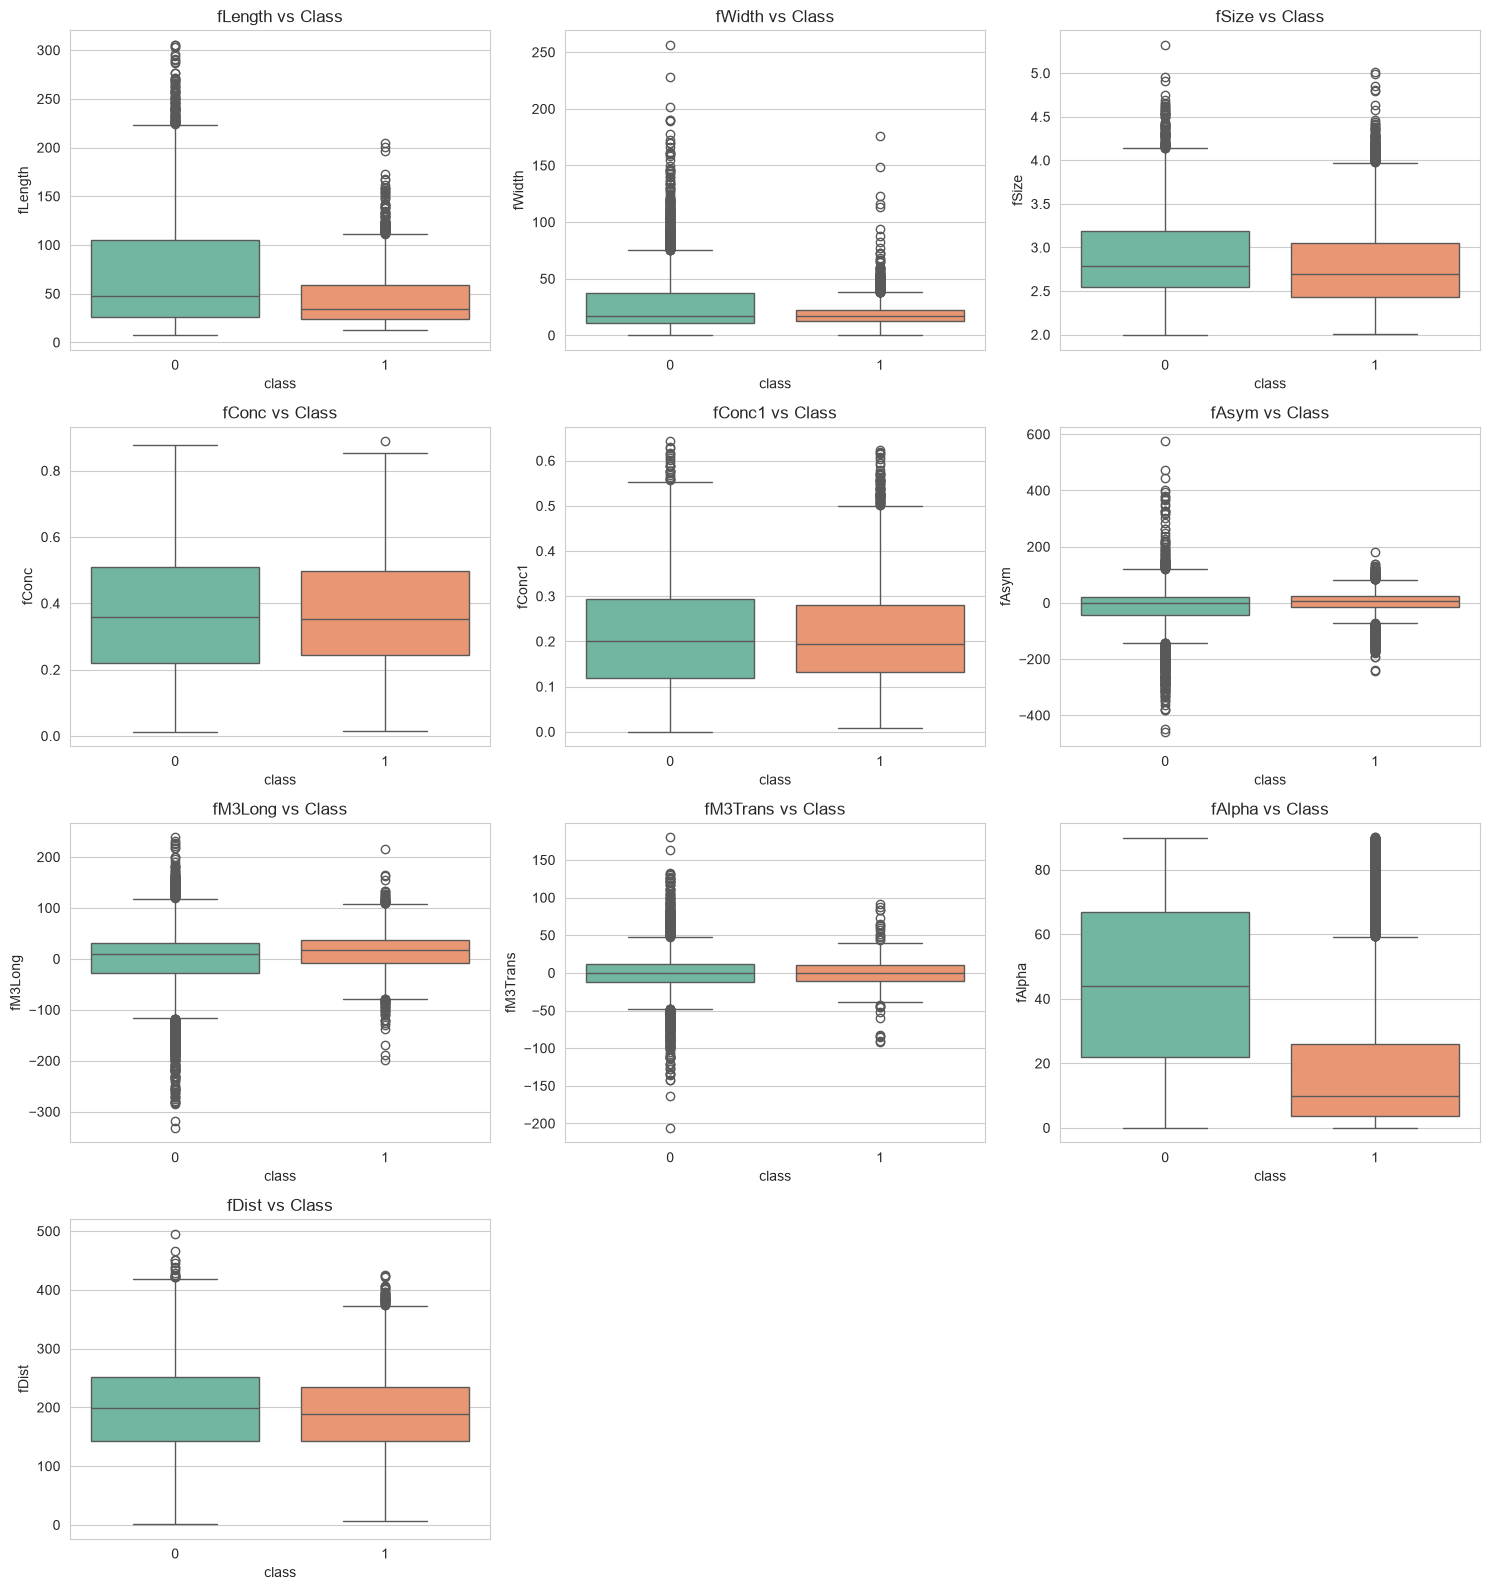
\includegraphics[width=0.95\textwidth]{eda_box}
\caption{Boxplot di ogni feature per classe (training set): \texttt{fAlpha} è la più discriminante, i momenti trasversali separano poco le classi.}
\label{fig:box}
\end{figure}

L'analisi della matrice di correlazione di Pearson (Figura~\ref{fig:corr}) 
evidenzia forti interdipendenze lineari tra alcune feature. Le variabili 
\texttt{fConc} e \texttt{fConc1} risultano pressoché colineari (correlazione di 
$0{,}98$) e presentano una marcata anticorrelazione con \texttt{fSize} 
($-0{,}85$ e $-0{,}81$). Anche il gruppo formato da \texttt{fLength}, 
\texttt{fWidth} e \texttt{fSize} mostra correlazioni significative, comprese tra
$0{,}70$ e $0{,}77$. Questa elevata ridondanza informativa implica che il 
degrado o l'assenza di una di queste feature possa essere parzialmente 
compensato dall'informazione contenuta nelle altre. In netto contrasto, 
\texttt{fAlpha} si conferma la variabile più discriminante ma risulta quasi del 
tutto scorrelata dal resto del dataset; di conseguenza, la sua informazione 
risulta unica e non vicariabile in caso di corruzione.

\begin{figure}[H]\centering
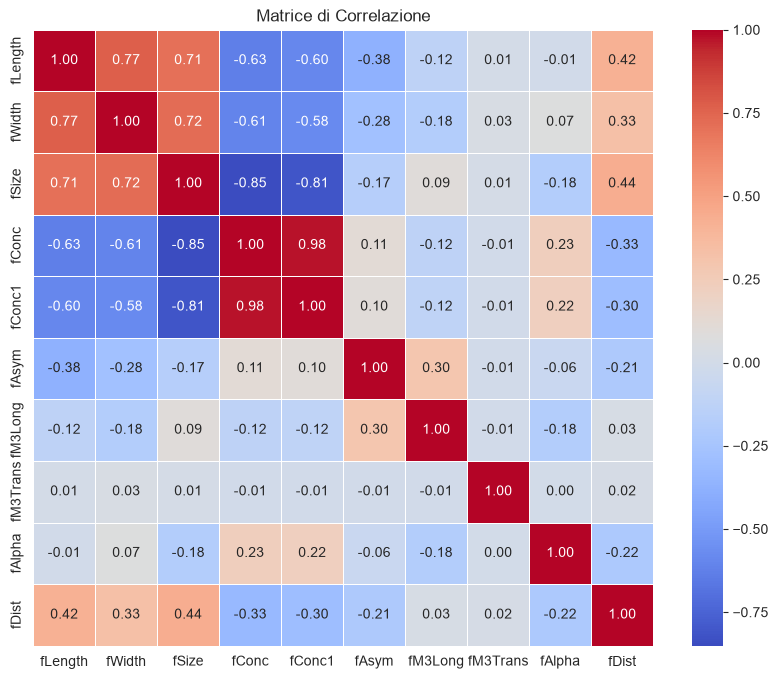
\includegraphics[width=0.82\textwidth]{eda_corr}
\caption{Matrice di correlazione tra le feature (training set). Spiccano la quasi-ridondanza \texttt{fConc}/\texttt{fConc1} e l'anticorrelazione di \texttt{fSize} con le concentrazioni; \texttt{fAlpha} è quasi scorrelata da tutte.}
\label{fig:corr}
\end{figure}

% ============================================================
% 5. PREPROCESSING
% ============================================================
\section{Preprocessing: standardizzazione}\label{sec:prep}

La notevole eterogeneità delle scale numeriche osservata durante l'analisi 
esplorativa rende indispensabile la standardizzazione delle feature (traslazione 
a media nulla e varianza unitaria). Questo passaggio è particolarmente critico 
per la stabilità e la convergenza delle reti neurali. In assenza di 
standardizzazione, le feature caratterizzate da magnitudo elevate dominerebbero 
l'aggiornamento dei gradienti esclusivamente in virtù della loro scala, e non 
per il loro effettivo potere predittivo.

Per garantire la rigorosità metodologica ed evitare il \textit{data leakage}, 
i parametri di scalatura (media e deviazione standard) sono stati estratti 
esclusivamente dal training set. Tali parametri sono stati successivamente 
applicati in modo immutato per trasformare il validation e il test set.

% ============================================================
% 6. MODELLI
% ============================================================
\section{Modelli}\label{sec:modelli}

Lo studio confronta tre modelli supervisionati, selezionati per rappresentare 
architetture dotate di livelli crescenti di tolleranza intrinseca al rumore. La 
Tabella~\ref{tab:modelli} ne riassume i parametri strutturali e gli iperparametri.

La \textbf{rete neurale Base} è un \textit{Multi-Layer Perceptron} (MLP) 
volutamente semplificato. L'architettura prevede in ingresso le dieci feature 
standardizzate, elaborate tramite due strati densi nascosti (rispettivamente da 
$32$ e $16$ neuroni, entrambi con funzione di attivazione ReLU). L'ultimo strato 
è costituito da un singolo neurone con attivazione sigmoide per la stima della 
probabilità di classe. L'addestramento sfrutta l'ottimizzatore Adam (tasso di 
apprendimento $10^{-3}$) e la funzione di costo \textit{binary cross-entropy}, 
per $75$ epoche con un batch size di $32$. Privo di alcun meccanismo di 
regolarizzazione, questo modello rappresenta la baseline "ingenua", in quanto è 
strutturalmente libero di adattarsi anche ai pattern spuri introdotti dal 
rumore (\textit{overfitting}).

La \textbf{rete neurale Pro} mantiene l'esatta architettura della rete Base ma 
integra quattro meccanismi specifici per contrastare l'overfitting. La 
regolarizzazione \emph{L2} (coefficiente $10^{-4}$ sui pesi degli strati nascosti) 
penalizza la magnitudo dei pesi, disincentivando confini decisionali 
eccessivamente complessi. Il \emph{dropout} (probabilità $0{,}2$) inibisce 
iterativamente frazioni casuali di neuroni, costringendo la rete a distribuire 
l'apprendimento ed evitare la dipendenza da singole unità. Il 
\emph{class weight} bilanciato incrementa la penalizzazione per gli errori 
commessi sulla classe minoritaria (adroni), bilanciando l'aggiornamento dei 
pesi. Infine, l'\emph{early stopping} monitora la funzione di costo sul 
validation set e interrompe l'addestramento in caso di assenza di miglioramenti 
per $15$ epoche consecutive (entro un limite massimo di $150$), ripristinando i 
pesi ottimali.

Il \textbf{Random Forest} è un \textit{ensemble} composto da $200$ alberi 
decisionali. La sua robustezza deriva dal principio del \textit{bagging}: le 
previsioni dei singoli alberi, ciascuno addestrato su sottoinsiemi casuali di 
dati e feature, vengono aggregate tramite voto maggioritario. Questo meccanismo 
tende a cancellare la varianza degli errori individuali. Poiché l'algoritmo non 
opera tramite ottimizzazione iterativa, non sono disponibili curve di 
apprendimento; le performance sono valutate unicamente tramite le metriche e la 
matrice di confusione finali.

\begin{table}[H]\centering\small
\caption{Parametri principali dei tre modelli confrontati.}\label{tab:modelli}
\begin{tabular}{@{}l p{4.6cm} p{6.8cm}@{}}
\toprule
\textbf{Modello} & \textbf{Architettura} & \textbf{Regolarizzazione / iperparametri} \\
\midrule
NN Base & Dense(32) $\to$ Dense(16) $\to$ sigmoide & nessuna; Adam $10^{-3}$, 75 epoche, batch 32 \\[4pt]
NN Pro & Dense(32) $\to$ Dense(16) $\to$ sigmoide & L2 $10^{-4}$, dropout 0,2, class weight bilanciato, early stopping (patience 15), max 150 epoche \\[4pt]
Random Forest & 200 alberi decisionali & aggregazione per voto, \texttt{random\_state}=42 \\
\bottomrule
\end{tabular}
\end{table}

Per la valutazione complessiva vengono utilizzate quattro metriche, calcolate sul 
test set pulito applicando una soglia decisionale di $0{,}5$. L'Accuratezza 
globale fornisce un'indicazione di massima, ma risulta limitata a causa dello 
sbilanciamento delle classi. Per compensare, vengono introdotte l'F1 macro e la 
Recall macro, che mediano le prestazioni attribuendo pari importanza a entrambe 
le classi, penalizzando severamente i modelli che tendono a ignorare gli adroni. 
Infine, l'AUC (\textit{Area Under the ROC Curve}) valuta la qualità intrinseca 
del \textit{ranking} probabilistico indipendentemente dalla soglia scelta.

% ============================================================
% 7. BASELINE
% ============================================================
\section{Baseline su dati puliti}\label{sec:baseline}

L'addestramento preliminare sui dati originali stabilisce il riferimento di 
prestazioni a livello $0\%$ di corruzione. Le metriche estratte fungono da 
standard di paragone per misurare quantitativamente i futuri degradi prestazionali. 
La Tabella~\ref{tab:baseline} riassume i risultati sul test set.

\begin{table}[H]\centering\small
\caption{Metriche di test dei tre modelli sui dati puliti (riferimento a 0\% di rumore).}\label{tab:baseline}
\begin{tabular}{lccc}
\toprule
\textbf{Modello} & \textbf{Accuratezza} & \textbf{F1 macro} & \textbf{AUC} \\
\midrule
NN Base       & 0,8678 & 0,8517 & 0,9214 \\
NN Pro        & 0,8601 & 0,8468 & 0,9238 \\
Random Forest & 0,8785 & 0,8629 & 0,9300 \\
\bottomrule
\end{tabular}
\end{table}

I modelli presentano prestazioni iniziali comparabili, con valori di accuratezza
compresi tra l'$86\%$ e l'$88\%$ e AUC tra $0{,}92$ e $0{,}93$. Il Random Forest
emerge come l'algoritmo più performante su tutte le metriche. L'accuratezza della
rete Pro risulta marginalmente inferiore a quella della rete Base; questa
flessione, però, non è imputabile principalmente a L2 e dropout, bensì al
\emph{class weight} bilanciato applicato con soglia decisionale fissa a $0{,}5$:
ribilanciando l'obiettivo a favore della classe minoritaria, la rete Pro
aumenta la recall sugli adroni (da $0{,}77$ a $0{,}80$) a scapito di una quota
di recall sui gamma, riducendo l'accuratezza globale senza intaccare la qualità
del \textit{ranking} probabilistico. Coerentemente, la rete Pro registra un'AUC
lievemente superiore rispetto alla Base — metrica indipendente dalla soglia — a
conferma di una maggiore solidità nell'ordinamento delle probabilità prodotte.

Le matrici di confusione (Figura~\ref{fig:base_cm}) illustrano il comportamento 
predittivo in presenza di classi sbilanciate. Tutti i classificatori isolano con 
efficacia il segnale (gamma), ma concentrano la maggioranza degli errori 
sull'identificazione degli adroni. Le \textit{learning curves} delle due reti 
(Figura~\ref{fig:base_curve}) indicano una convergenza regolare. Il divario 
limitato tra le metriche di training e validation conferma l'assenza di un marcato 
\textit{overfitting} sui dati non alterati per entrambe le architetture.

\begin{figure}[H]\centering
\begin{minipage}{0.32\textwidth}\centering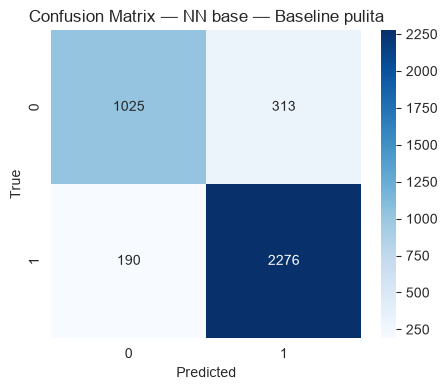
\includegraphics[width=\textwidth]{baseline_nnbase_cm}\end{minipage}\hfill
\begin{minipage}{0.32\textwidth}\centering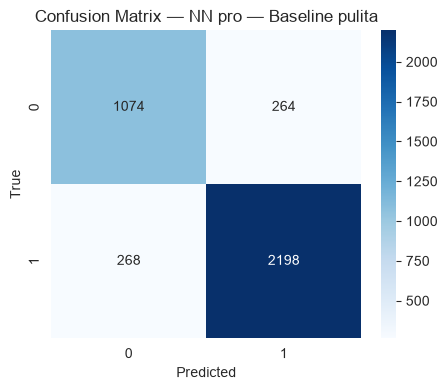
\includegraphics[width=\textwidth]{baseline_nnpro_cm}\end{minipage}\hfill
\begin{minipage}{0.32\textwidth}\centering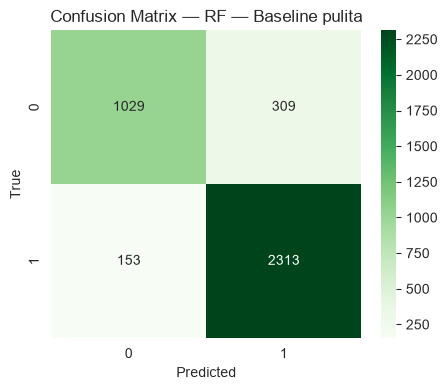
\includegraphics[width=\textwidth]{baseline_rf_cm}\end{minipage}
\caption{Matrici di confusione sui dati puliti: rete Base, rete Pro e Random Forest (da sinistra a destra). Tutti riconoscono bene i gamma, gli errori si concentrano sugli adroni.}
\label{fig:base_cm}
\end{figure}

\begin{figure}[H]\centering
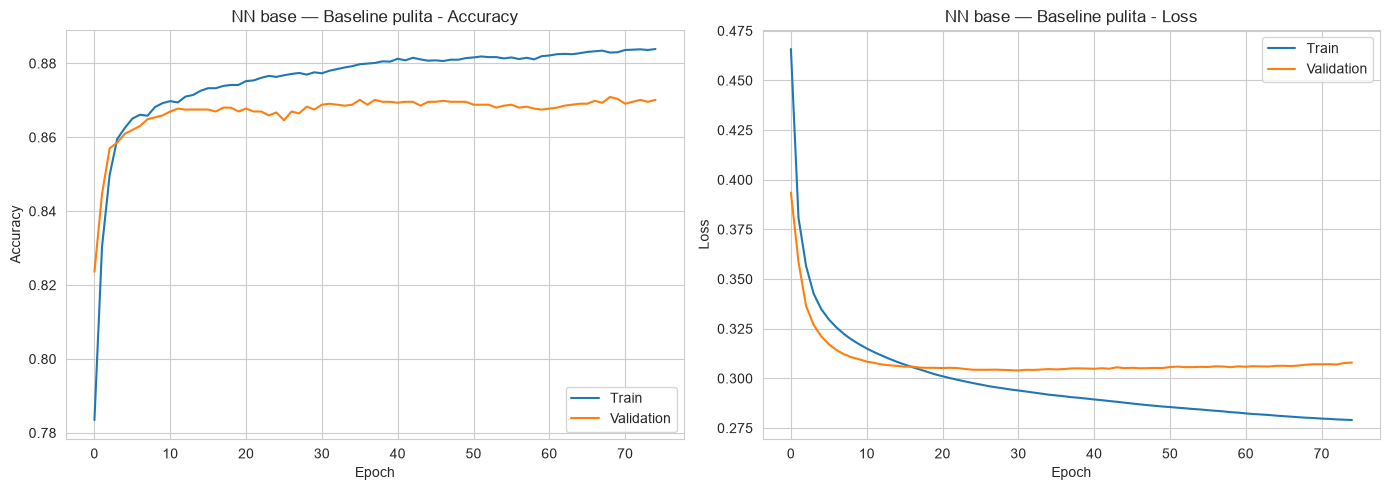
\includegraphics[width=0.9\textwidth]{baseline_nnbase_curve}\\[8pt]
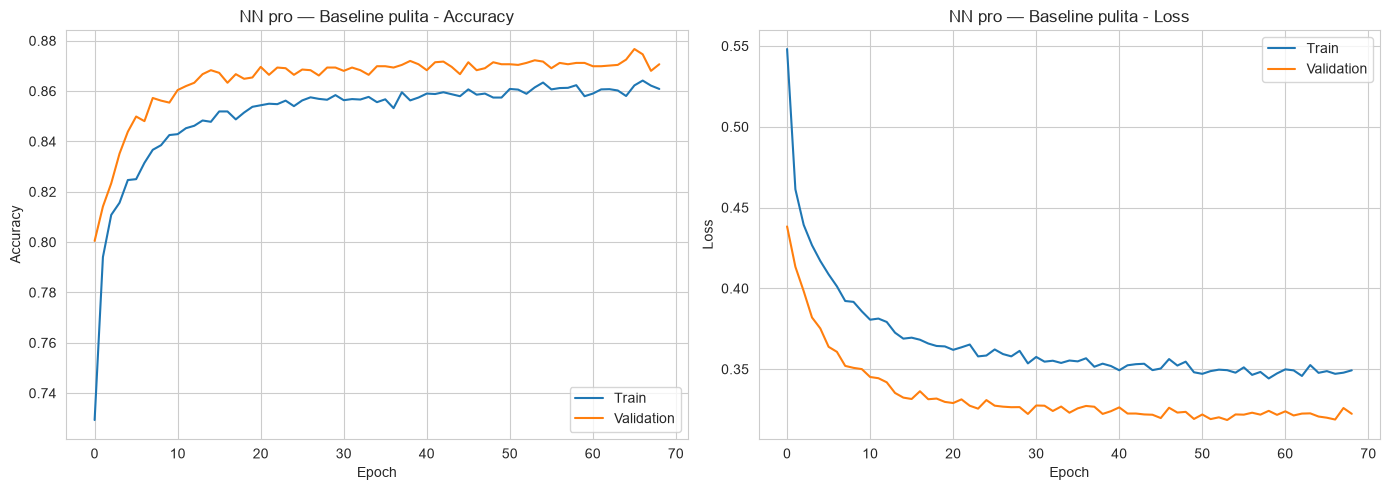
\includegraphics[width=0.9\textwidth]{baseline_nnpro_curve}
\caption{Curve di accuratezza e loss (train vs validation) sui dati puliti: rete Base (in alto) e rete Pro (in basso).}
\label{fig:base_curve}
\end{figure}

L'estrazione della \textit{feature importance} tramite Random Forest 
(Figura~\ref{fig:featimp}) conferma quantitativamente le ipotesi formulate 
nell'analisi esplorativa. La feature \texttt{fAlpha} domina lo spazio predittivo
con un valore di importanza prossimo a $0{,}24$, circa una volta e mezza il
secondo parametro più rilevante (\texttt{fLength}, $\approx 0{,}15$). Seguono in
ordine decrescente \texttt{fLength}, \texttt{fWidth} e \texttt{fSize}.

\begin{figure}[H]\centering
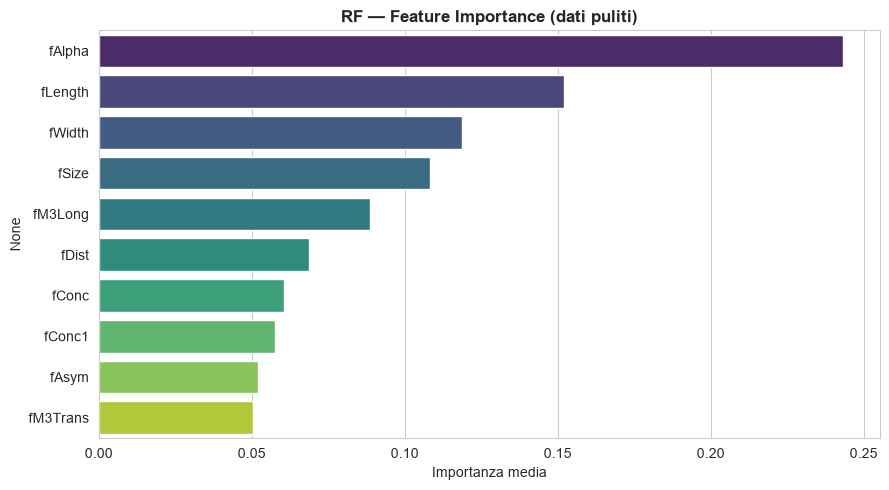
\includegraphics[width=0.86\textwidth]{baseline_featimp}
\caption{Importanza delle feature secondo il Random Forest sui dati puliti. \texttt{fAlpha} domina, coerentemente con la separabilità osservata nei boxplot.}
\label{fig:featimp}
\end{figure}

% ============================================================
% 8. METODOLOGIA DEL RUMORE
% ============================================================
\section{Metodologia di iniezione del rumore}\label{sec:rumore}

Il rumore altera esclusivamente il training set, mantenendo intatti validation e 
test set. Questo approccio garantisce di valutare in modo corretto la 
generalizzazione di un modello addestrato su dati imperfetti. Per ogni rumore, i 
modelli sono riaddestrati iterativamente su tre livelli di intensità ($10\%$, 
$25\%$, $40\%$), valutando poi le performance sempre sul medesimo test set. 
L'iniezione del rumore avviene sul training set già standardizzato: essendo le 
perturbazioni additive o monotone, l'operazione equivale matematicamente a 
corrompere i dati originali e standardizzarli in un secondo momento.

Si definiscono sette meccanismi di corruzione:

\subsection{I sette tipi di rumore}

\paragraph{Feature noise (rumore gaussiano).} A ogni singola feature del 
training set viene sommato un rumore bianco gaussiano, caratterizzato da media 
nulla e deviazione standard proporzionale al livello percentuale scelto. Poiché 
le variabili sono state preventivamente standardizzate, l'applicazione di un 
rumore al livello $40\%$ equivale a introdurre fluttuazioni pari al $40\%$ 
della deviazione standard nativa di ciascuna feature.

\paragraph{Feature noise localizzato.} In questo scenario, l'intensità del 
rumore viene mantenuta costante a $\sigma = 0{,}35$, variando invece il numero 
di feature perturbate. La selezione avviene in base alla gerarchia di importanza 
stabilita. Al livello $10\%$ il disturbo altera unicamente \texttt{fAlpha}; al 
$25\%$ coinvolge le prime tre variabili discriminanti; al $40\%$ l'iniezione 
si estende alle prime cinque.

\paragraph{Label noise random.} Una percentuale di osservazioni del training set 
pari al livello selezionato subisce l'inversione della variabile target (da $0$ 
a $1$ e viceversa). Il campionamento avviene in maniera puramente casuale, 
simulando errori di annotazione distribuiti uniformemente.

\paragraph{Label noise borderline.} L'inversione delle etichette si concentra 
sulle istanze topologicamente più ambigue. Dopo aver calcolato i centroidi delle 
due classi nello spazio multidimensionale standardizzato, si misura la distanza 
di ogni campione dal centroide della classe opposta. L'inversione colpisce 
esclusivamente i campioni caratterizzati da distanza minima, ovvero quelli 
posizionati in stretta prossimità del confine decisionale ottimale.

\paragraph{Missing values.} Singole misurazioni vengono eliminate e sostituite 
con un valore nullo (\texttt{NaN}), trattando ogni cella della matrice come 
evento indipendente con probabilità pari al livello di corruzione. Non potendo 
i modelli elaborare dati incompleti, si impone l'uso di un'imputazione: in 
questa sede vengono confrontate l'imputazione per media e per mediana della 
rispettiva feature.

\paragraph{Outlier.} Un numero di campioni proporzionale al livello 
selezionato subisce una corruzione massiva: tutti i valori delle feature per la 
riga scelta vengono sostituiti da parametri estremi (fissati a $\pm 5$ 
deviazioni standard, con attribuzione casuale del segno). Le strategie di 
mitigazione esplorate sono tre: lasciare le istanze inalterate; applicare la 
\textit{winsorizzazione} (troncamento dei valori limite in corrispondenza dei 
percentili al $5\%$ e $95\%$) per contenere la magnitudo estrema; imputare i 
dati, marcando come mancanti le istanze con z-score assoluto maggiore di $4$ 
e sostituendole con la mediana. Come riferimento primario verrà utilizzata 
la winsorizzazione, in virtù del suo bilanciamento tra robustezza e 
conservazione dei dati.

\paragraph{Missing feature (sensore guasto).} Intere colonne di feature 
vengono azzerate su tutti i sottoinsiemi (training, validation e test), 
simulando il totale fallimento sistemico di un sensore. Anche in questo caso 
la rimozione procede seguendo la gerarchia di importanza decrescente. Al 
$10\%$ viene inibita l'elaborazione di \texttt{fAlpha}, al $25\%$ si 
azzerano le prime tre variabili predittive, fino alle prime cinque al $40\%$. 
Questo approccio impone condizioni volutamente pessimistiche, sopprimendo le 
fonti informative primarie.

% ============================================================
% 9. RISULTATI PER TIPO DI RUMORE
% ============================================================
\section{Risultati per tipo di rumore}\label{sec:risultati}

L'impatto dei sette disturbi viene analizzato singolarmente, quantificando il 
degrado prestazionale al crescere della corruzione. Per ciascun test vengono 
forniti i prospetti delle metriche misurate sui vari step e le comparazioni 
grafiche sull'andamento dell'accuratezza globale e dell'F1 macro. L'analisi 
è integrata, dove necessario, dallo studio delle learning curves e dalle 
matrici di confusione inerenti allo scenario estremo.

% ---------- 9.1 Feature noise ----------
\subsection{Feature noise}

L'aggiunta di rumore bianco gaussiano sulle feature produce un degrado morbido 
e progressivo. Come riportato nella Tabella~\ref{tab:fn}, anche al massimo 
livello di corruzione ($40\%$) l'accuratezza di tutti i modelli si preserva 
al di sopra dell'$83\%$, registrando una flessione limitata a tre o quattro 
punti percentuali rispetto alla baseline. I grafici prestazionali 
(Figura~\ref{fig:fn_acc}) restituiscono curve con pendenza lieve e omogenea 
sia in termini di accuratezza sia per quanto riguarda l'F1 macro.

\begin{table}[H]\centering\footnotesize
\setlength{\tabcolsep}{4pt}
\caption{Feature noise: metriche al variare del livello di rumore (test set). R$_m$ = recall macro.}\label{tab:fn}
\begin{tabular}{c *{12}{c}}
\toprule
 & \multicolumn{4}{c}{NN Base} & \multicolumn{4}{c}{NN Pro} & \multicolumn{4}{c}{Random Forest}\\
\cmidrule(lr){2-5}\cmidrule(lr){6-9}\cmidrule(lr){10-13}
Rumore & Acc & R$_m$ & F1$_m$ & AUC & Acc & R$_m$ & F1$_m$ & AUC & Acc & R$_m$ & F1$_m$ & AUC \\
\midrule
Pulito & 0.8678 & 0.84 & 0.85 & 0.9214 & 0.8601 & 0.85 & 0.85 & 0.9238 & 0.8785 & 0.85 & 0.86 & 0.9300 \\
10\% & 0.8657 & 0.84 & 0.85 & 0.9187 & 0.8636 & 0.85 & 0.85 & 0.9204 & 0.8646 & 0.83 & 0.84 & 0.9222 \\
25\% & 0.8520 & 0.81 & 0.83 & 0.9074 & 0.8465 & 0.83 & 0.83 & 0.9071 & 0.8494 & 0.81 & 0.82 & 0.9041 \\
40\% & 0.8328 & 0.78 & 0.80 & 0.8941 & 0.8417 & 0.82 & 0.82 & 0.8940 & 0.8318 & 0.78 & 0.80 & 0.8913 \\
\bottomrule
\end{tabular}
\end{table}


\begin{figure}[H]\centering
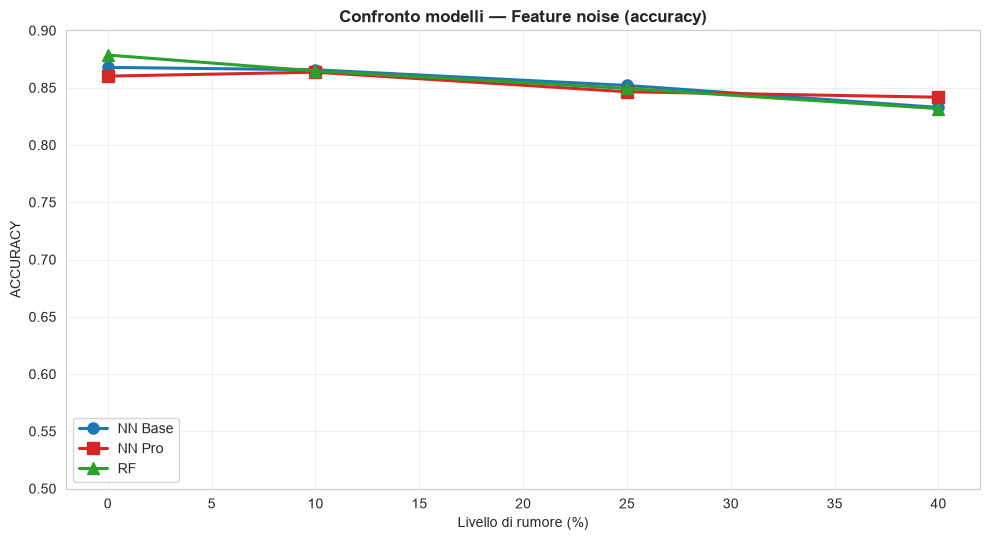
\includegraphics[width=0.86\textwidth]{fn_compare_acc}\\[8pt]
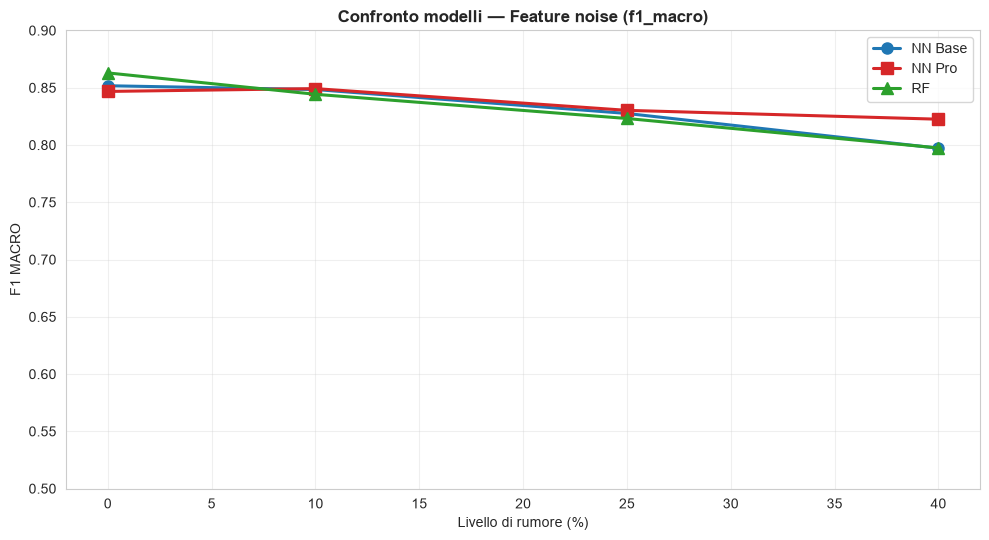
\includegraphics[width=0.86\textwidth]{fn_compare_f1}
\caption{Feature noise: accuratezza (in alto) e F1 macro (in basso) dei tre modelli al crescere del rumore.}
\label{fig:fn_acc}
\end{figure}

Al livello $40\%$, la rete Pro raggiunge il primato assoluto ($0{,}8417$), 
distaccando sia la rete Base ($0{,}8328$) sia il Random Forest ($0{,}8318$). 
Questo risultato conferma l'efficacia dei sistemi di regolarizzazione di fronte 
a input instabili: la sinergia tra penalizzazione L2 e dropout funge da filtro, 
impedendo all'architettura di modellare e apprendere le fluttuazioni stocastiche 
introdotte. La rete Base, al contrario, mancando di vincoli strutturali, tende 
ad assecondare il rumore, peggiorando le proprie capacità di classificazione 
su campioni ignoti. Nelle curve di apprendimento relative allo scenario estremo 
(Figura~\ref{fig:fn_curve}) si nota come la rete Base conservi un costante, 
seppur ridotto, gap tra training e validation loss; la rete Pro, di contro, 
mantiene le curve di training e validation costantemente appaiate. A livello 
generale, la marcata ridondanza interna tra le feature attenua fortemente 
l'impatto distruttivo, consentendo all'algoritmo di dedurre parzialmente 
le informazioni corrotte dalle variabili adiacenti correlate.

\begin{figure}[H]\centering
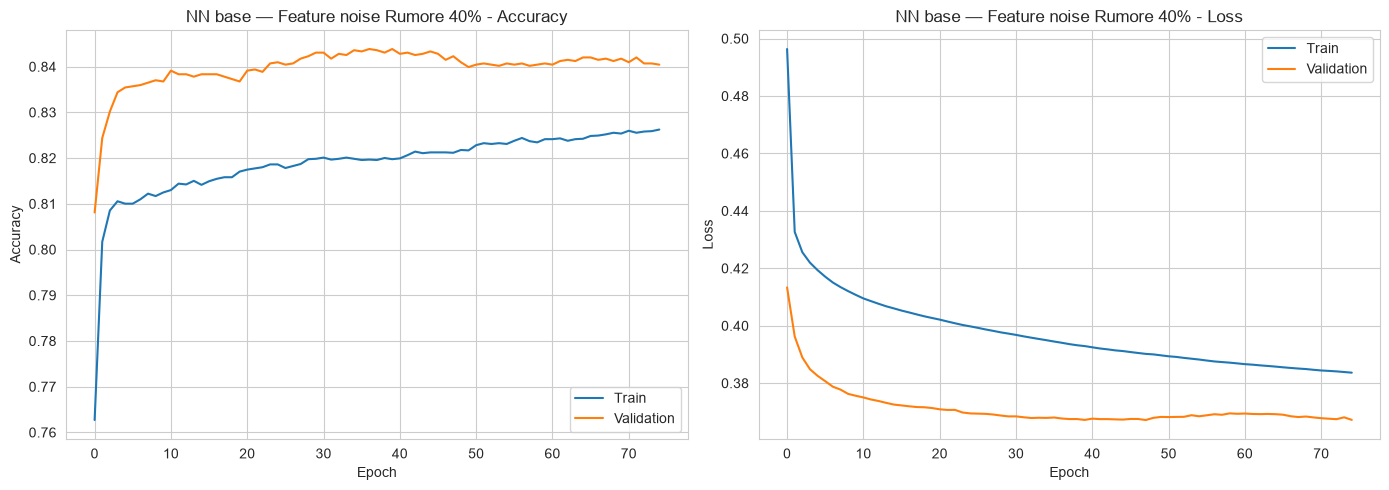
\includegraphics[width=0.9\textwidth]{fn_nnbase_curve40}\\[8pt]
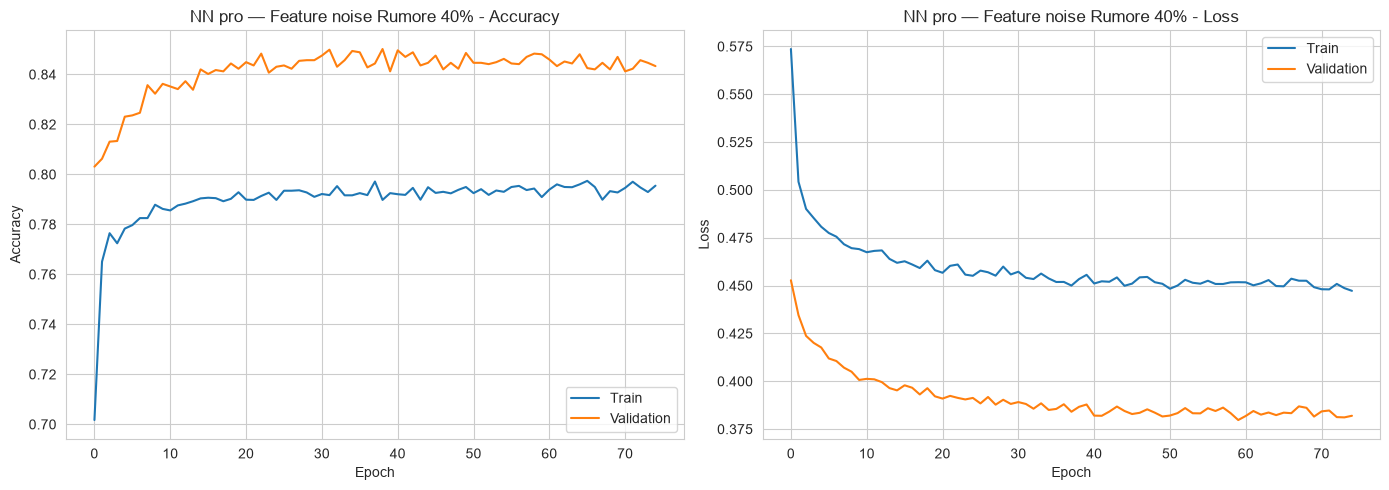
\includegraphics[width=0.9\textwidth]{fn_nnpro_curve40}
\caption{Feature noise al 40\%: curve di addestramento della rete Base (in alto) e della rete Pro (in basso). Nella rete Pro train e validation restano sovrapposte: la regolarizzazione evita l'adattamento al rumore.}
\label{fig:fn_curve}
\end{figure}

Il decadimento delle performance risulta, tuttavia, asimmetrico. In presenza di 
uno sbilanciamento di classe, i modelli tendono a preservare un'accuratezza 
globale elevata sacrificando il potere predittivo sulla classe rara. Al $40\%$ 
di rumore, la \textit{recall} per la classe minoritaria (adroni) della rete Base 
precipita da $0{,}77$ a $0{,}59$, in netto contrasto con la \textit{recall} dei 
gamma che si incrementa da $0{,}92$ a $0{,}97$. Questa discrepanza evidenzia la 
tendenza dell'algoritmo a declassificare i campioni adronici incerti e ad 
assorbirli erroneamente nella classe maggioritaria. L'implementazione del 
\emph{class weight} all'interno della rete Pro argina tale fenomeno, sostenendo 
la recall adronica a $0{,}73$. Le matrici di confusione generate dalla rete Base 
(Figura~\ref{fig:fn_progress}) quantificano inequivocabilmente tale scivolamento.

\begin{figure}[H]\centering
\begin{minipage}{0.32\textwidth}\centering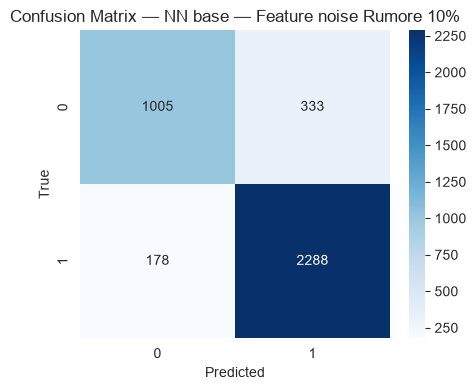
\includegraphics[width=\textwidth]{fn_nnbase_cm10}\end{minipage}\hfill
\begin{minipage}{0.32\textwidth}\centering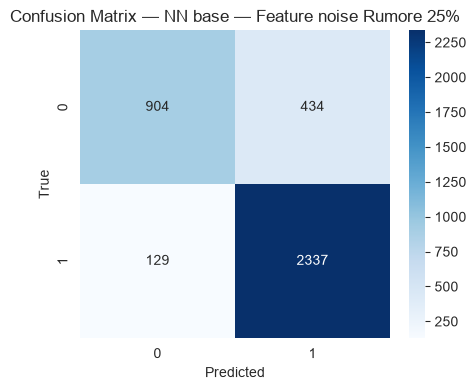
\includegraphics[width=\textwidth]{fn_nnbase_cm25}\end{minipage}\hfill
\begin{minipage}{0.32\textwidth}\centering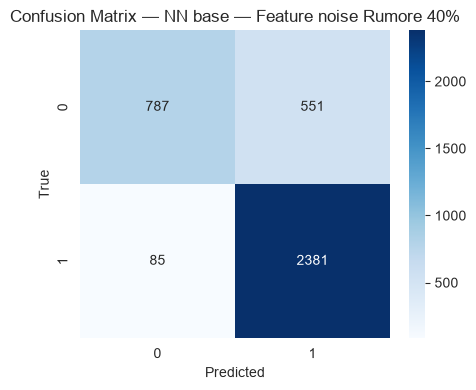
\includegraphics[width=\textwidth]{fn_nnbase_cm40}\end{minipage}
\caption{Feature noise, rete Base: matrici di confusione al 10\%, 25\% e 40\% (da sinistra a destra). Gli adroni (riga 0) vengono classificati come gamma con frequenza crescente.}
\label{fig:fn_progress}
\end{figure}

% ---------- 9.1bis Feature noise localizzato ----------
\subsection{Feature noise localizzato}

Selezionando con precisione le fonti di corruzione invece di spalmare il rumore 
globalmente, l'impatto predittivo non subisce drammatici stravolgimenti 
(Tabella~\ref{tab:fnloc}). L'intensità della perturbazione rimane costante a 
$\sigma = 0{,}35$.

\begin{table}[H]\centering\footnotesize
\setlength{\tabcolsep}{4pt}
\caption{Feature noise localizzato ($\sigma = 0{,}35$) sulle sole feature più importanti: il livello indica quante feature sono colpite (10\%$\to$top-1, 25\%$\to$top-3, 40\%$\to$top-5). R$_m$ = recall macro.}\label{tab:fnloc}
\begin{tabular}{c *{12}{c}}
\toprule
 & \multicolumn{4}{c}{NN Base} & \multicolumn{4}{c}{NN Pro} & \multicolumn{4}{c}{Random Forest}\\
\cmidrule(lr){2-5}\cmidrule(lr){6-9}\cmidrule(lr){10-13}
Rumore & Acc & R$_m$ & F1$_m$ & AUC & Acc & R$_m$ & F1$_m$ & AUC & Acc & R$_m$ & F1$_m$ & AUC \\
\midrule
Pulito & 0.8678 & 0.84 & 0.85 & 0.9214 & 0.8601 & 0.85 & 0.85 & 0.9238 & 0.8785 & 0.85 & 0.86 & 0.9300 \\
10\% & 0.8651 & 0.84 & 0.85 & 0.9211 & 0.8651 & 0.85 & 0.85 & 0.9243 & 0.8743 & 0.85 & 0.86 & 0.9274 \\
25\% & 0.8523 & 0.82 & 0.83 & 0.9043 & 0.8478 & 0.83 & 0.83 & 0.9058 & 0.8533 & 0.82 & 0.83 & 0.9056 \\
40\% & 0.8452 & 0.81 & 0.82 & 0.8991 & 0.8386 & 0.82 & 0.82 & 0.8973 & 0.8389 & 0.79 & 0.81 & 0.8931 \\
\bottomrule
\end{tabular}
\end{table}


\begin{figure}[H]\centering
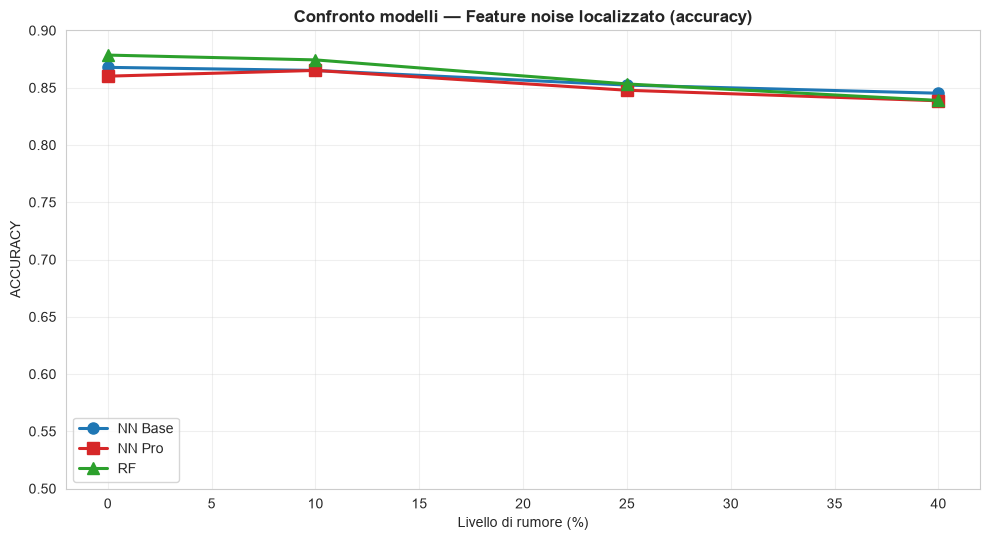
\includegraphics[width=0.86\textwidth]{fnloc_compare_acc}\\[8pt]
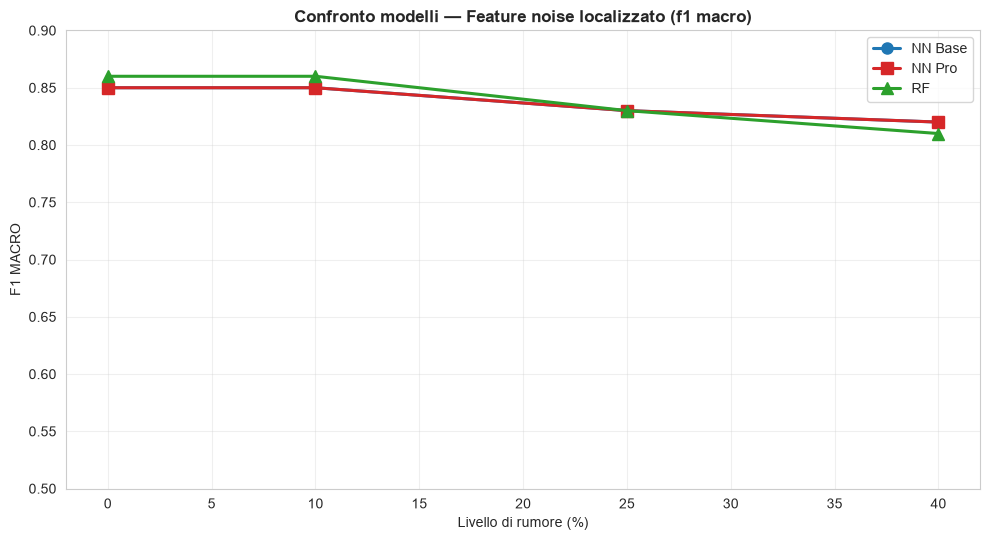
\includegraphics[width=0.86\textwidth]{fnloc_compare_f1}
\caption{Feature noise localizzato: accuratezza (in alto) e F1 macro (in basso). Le curve restano vicine e quasi piatte.}
\label{fig:fnloc_acc}
\end{figure}

Il decadimento si conferma lieve anche a fronte della perturbazione mirata sulle 
cinque feature fondamentali. Al livello $40\%$, tutti i classificatori si 
preservano sopra la soglia dell'$83\%$ in termini di accuratezza. L'analisi di 
classe (Figura~\ref{fig:fnloc_cm}) rimarca le dinamiche asimmetriche indagate 
precedentemente: al livello apicale, la recall adronica della rete Base staziona 
a $0{,}67$, mentre l'applicazione dei pesi sbilanciati nella rete Pro la 
sostiene al $0{,}75$.

L'andamento delle \textit{learning curves} non discosta da quanto evidenziato 
nel rumore diffuso (Figura~\ref{fig:fnloc_curve}). Il confronto concettuale 
più significativo emerge mettendolo in relazione con la completa omissione delle 
feature (missing feature): inficiare l'integrità di \texttt{fAlpha} riduce 
l'accuratezza della rete Base a $0{,}8651$, laddove la sua completa soppressione 
ne cagionerà il crollo a $0{,}8215$. La perturbazione degrada la qualità 
informativa ma non l'annulla, consentendo alla rete di attingere, mediante 
sistemi complessi di compensazione, a porzioni della geometria originale dei dati.

\begin{figure}[H]\centering
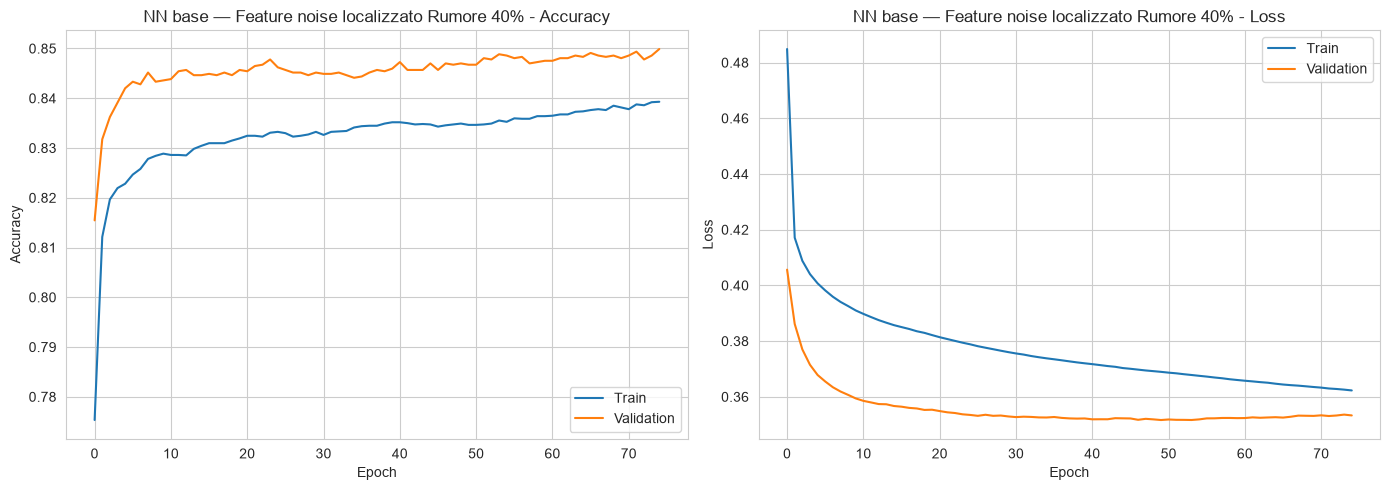
\includegraphics[width=0.9\textwidth]{fnloc_nnbase_curve40}\\[8pt]
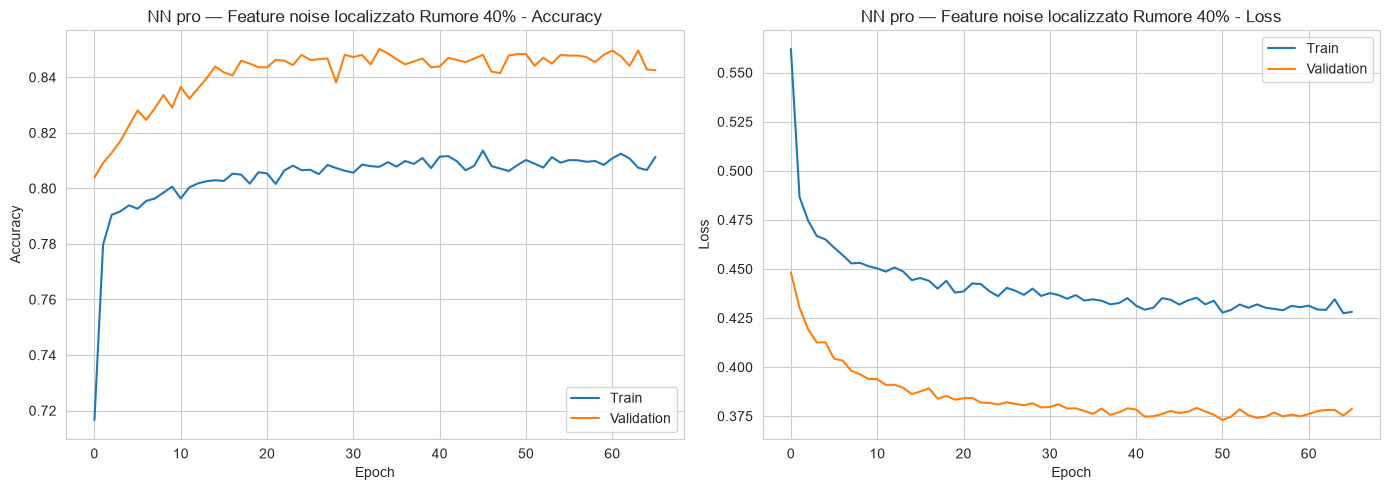
\includegraphics[width=0.9\textwidth]{fnloc_nnpro_curve40}
\caption{Feature noise localizzato al 40\%: curve di addestramento. L'andamento ricalca il feature noise globale, senza overfitting.}
\label{fig:fnloc_curve}
\end{figure}

\begin{figure}[H]\centering
\begin{minipage}{0.49\textwidth}\centering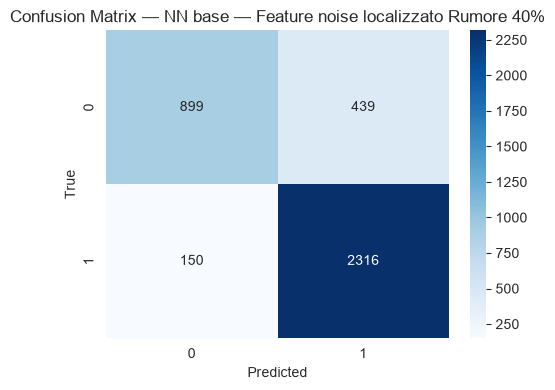
\includegraphics[width=\textwidth]{fnloc_nnbase_cm40}\end{minipage}\hfill
\begin{minipage}{0.49\textwidth}\centering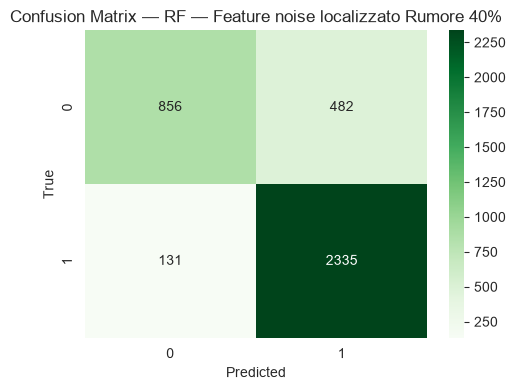
\includegraphics[width=\textwidth]{fnloc_rf_cm40}\end{minipage}
\caption{Feature noise localizzato al 40\%: matrici di confusione della rete Base (sinistra) e del Random Forest (destra).}
\label{fig:fnloc_cm}
\end{figure}

% ---------- 9.2 Label noise random ----------
\subsection{Label noise random}

L'alterazione stocastica della variabile target innesca dinamiche prestazionali 
nettamente dissimili da quelle viste sulle alterazioni continue. Fino alla soglia 
del $25\%$, i classificatori riescono a preservare metriche adeguate, ma subiscono 
un cedimento drammatico raggiunto il $40\%$. Come evincibile dalla 
Tabella~\ref{tab:lnr}, l'accuratezza della rete Base collassa a $0{,}7419$, 
seguita dal declino del Random Forest a $0{,}7179$. La rete Pro manifesta 
un'elevata resilienza strutturale, mantenendo l'accuratezza al $0{,}8044$ 
(Figura~\ref{fig:lnr_acc}).

\begin{table}[H]\centering\footnotesize
\setlength{\tabcolsep}{4pt}
\caption{Label noise random: metriche al variare del livello di rumore (test set). R$_m$ = recall macro.}\label{tab:lnr}
\begin{tabular}{c *{12}{c}}
\toprule
 & \multicolumn{4}{c}{NN Base} & \multicolumn{4}{c}{NN Pro} & \multicolumn{4}{c}{Random Forest}\\
\cmidrule(lr){2-5}\cmidrule(lr){6-9}\cmidrule(lr){10-13}
Rumore & Acc & R$_m$ & F1$_m$ & AUC & Acc & R$_m$ & F1$_m$ & AUC & Acc & R$_m$ & F1$_m$ & AUC \\
\midrule
Pulito & 0.8678 & 0.84 & 0.85 & 0.9214 & 0.8601 & 0.85 & 0.85 & 0.9238 & 0.8785 & 0.85 & 0.86 & 0.9300 \\
10\% & 0.8623 & 0.83 & 0.84 & 0.9128 & 0.8570 & 0.84 & 0.84 & 0.9200 & 0.8767 & 0.85 & 0.86 & 0.9214 \\
25\% & 0.8410 & 0.82 & 0.82 & 0.8882 & 0.8378 & 0.83 & 0.83 & 0.9081 & 0.8399 & 0.81 & 0.82 & 0.8884 \\
40\% & 0.7419 & 0.68 & 0.69 & 0.7513 & 0.8044 & 0.79 & 0.79 & 0.8677 & 0.7179 & 0.70 & 0.70 & 0.7673 \\
\bottomrule
\end{tabular}
\end{table}


\begin{figure}[H]\centering
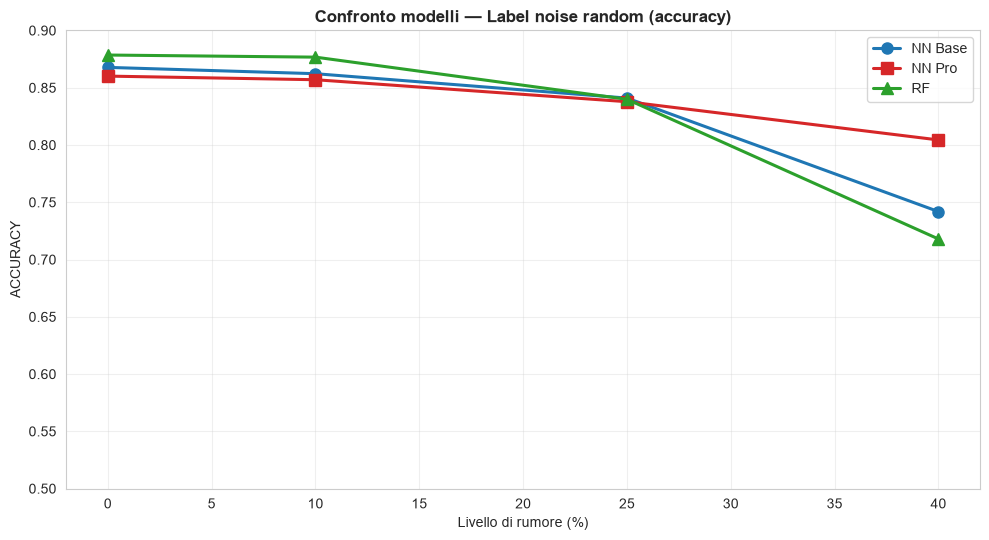
\includegraphics[width=0.86\textwidth]{lnr_compare_acc}\\[8pt]
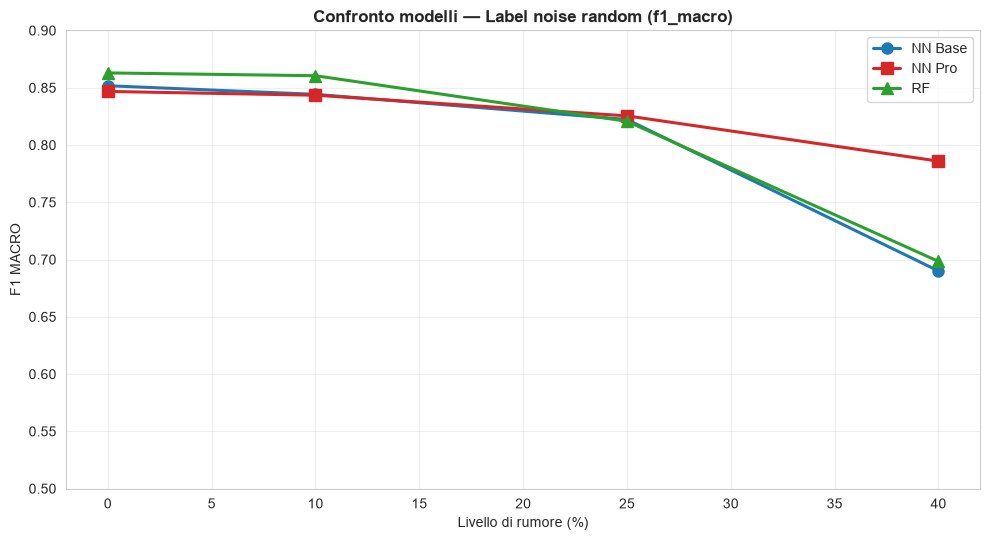
\includegraphics[width=0.86\textwidth]{lnr_compare_f1}
\caption{Label noise random: accuratezza e F1 macro. Al 40\% la rete Pro si stacca verso l'alto, mentre Base e Random Forest crollano.}
\label{fig:lnr_acc}
\end{figure}

La causa scatenante di questa severa divergenza si manifesta chiaramente nelle 
\textit{learning curves} (Figura~\ref{fig:lnr_curve}). Il processo di 
ottimizzazione della rete Base interiorizza le annotazioni spurie, portando la 
curva di training a sfiorare un inverosimile $88\%$, affiancata da un costante 
deterioramento della validation loss misurata sulle label originarie e pulite. 
In contrapposizione, l'\textit{early stopping} inserito nella rete Pro, 
monitorando i gradienti estratti dai dati non corrotti (validation test), 
interrompe tempestivamente l'iterazione. L'arresto preventivo blocca i pesi del 
percettrone a uno stadio prematuro ma ottimale, proteggendo il modello dalla 
fase critica di memorizzazione di massa del rumore, conservando una validation 
accuracy vicina all'$82\%$.

\begin{figure}[H]\centering
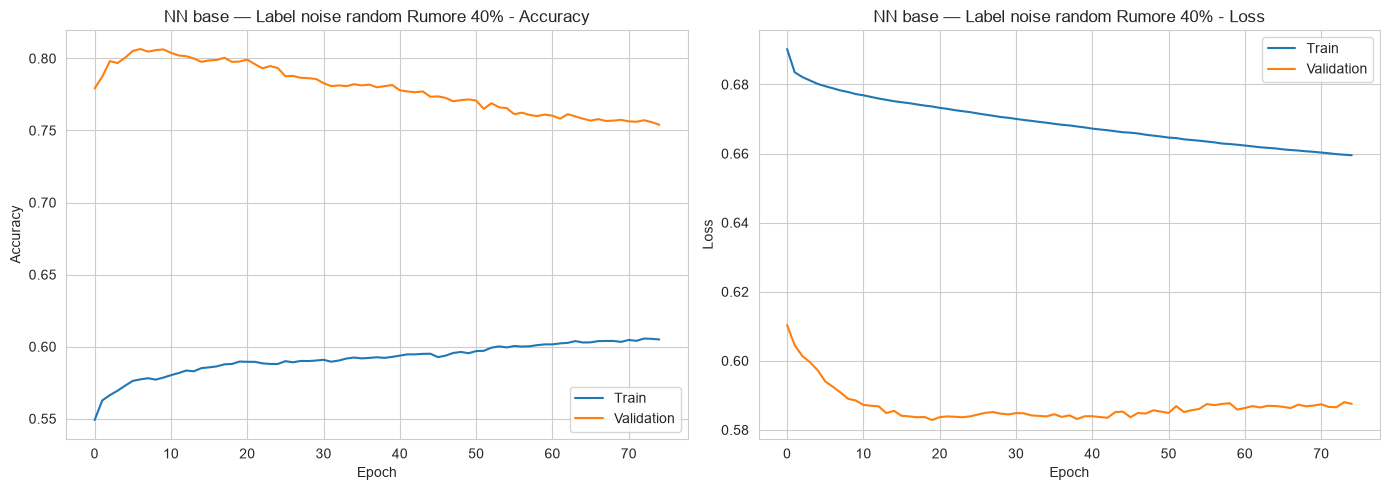
\includegraphics[width=0.9\textwidth]{lnr_nnbase_curve40}\\[8pt]
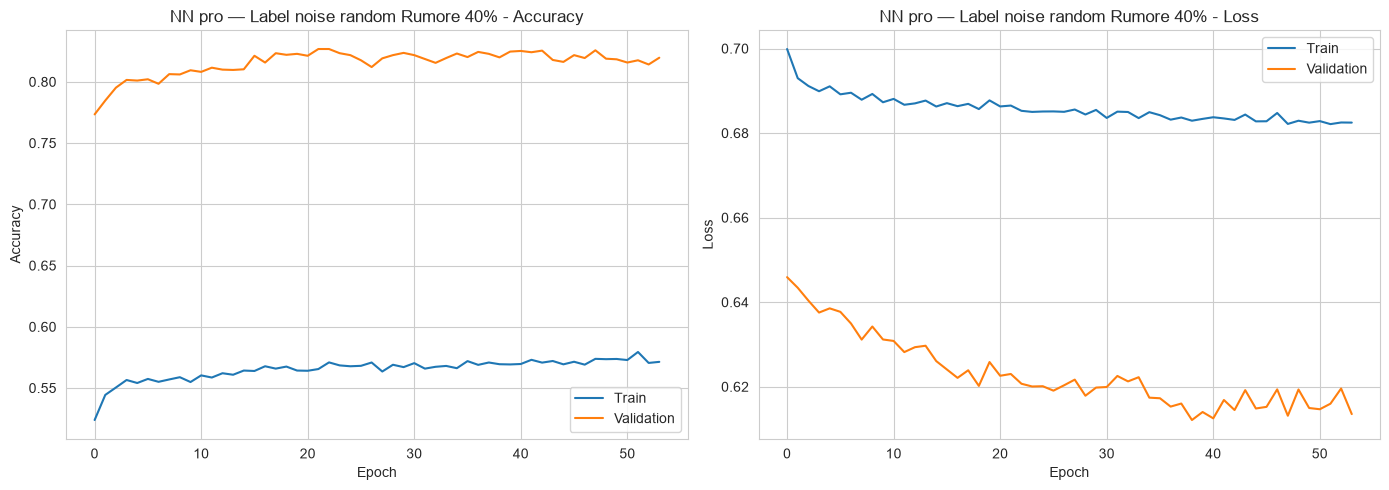
\includegraphics[width=0.9\textwidth]{lnr_nnpro_curve40}
\caption{Label noise random al 40\%: la Base memorizza le etichette corrotte (train sale, validation scende); la Pro, fermata dall'early stopping, mantiene alta la validation.}
\label{fig:lnr_curve}
\end{figure}

Essendo sprovvisto di meccanismi iterativi vincolati a set di validazione puri, 
il Random Forest assimila i falsi target all'interno dei nodi divisionali. La 
distribuzione indifferenziata dell'errore (Figura~\ref{fig:lnr_cm}) corrobora 
questa ipotesi, portando a decrementi paritari sulle metriche associate alle 
singole classi.

\begin{figure}[H]\centering
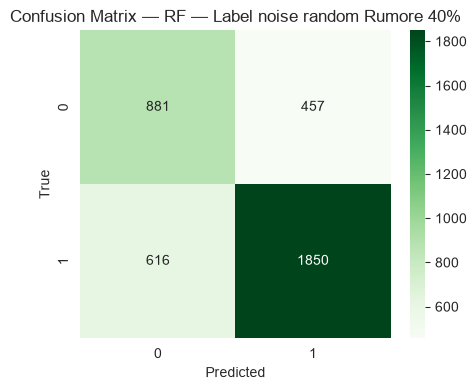
\includegraphics[width=0.52\textwidth]{lnr_rf_cm40}
\caption{Label noise random al 40\%: matrice di confusione del Random Forest. Gli errori aumentano su entrambe le classi.}
\label{fig:lnr_cm}
\end{figure}

% ---------- 9.3 Label noise borderline ----------
\subsection{Label noise borderline}

La corruzione selettiva delle istanze collocate ai margini dei confini 
decisionali costituisce l'anomalia maggiormente distruttiva per i modelli 
predittivi testati. Le metriche palesano un calo marcato già a fronte di 
variazioni contenute ($25\%$). Al raggiungimento del livello estremo ($40\%$),
le misurazioni collassano verso una quota di accuratezza approssimabile al
$60\%$, che scende perfino al di sotto della soglia di un classificatore inerte
che prevede sempre la classe maggioritaria ($\approx 65\%$): il rumore
borderline rende dunque i modelli attivamente fuorvianti
(Tabella~\ref{tab:lnb} e Figura~\ref{fig:lnb_acc}).

\begin{table}[H]\centering\footnotesize
\setlength{\tabcolsep}{4pt}
\caption{Label noise borderline: metriche al variare del livello di rumore (test set). R$_m$ = recall macro.}\label{tab:lnb}
\begin{tabular}{c *{12}{c}}
\toprule
 & \multicolumn{4}{c}{NN Base} & \multicolumn{4}{c}{NN Pro} & \multicolumn{4}{c}{Random Forest}\\
\cmidrule(lr){2-5}\cmidrule(lr){6-9}\cmidrule(lr){10-13}
Rumore & Acc & R$_m$ & F1$_m$ & AUC & Acc & R$_m$ & F1$_m$ & AUC & Acc & R$_m$ & F1$_m$ & AUC \\
\midrule
Pulito & 0.8678 & 0.84 & 0.85 & 0.9214 & 0.8601 & 0.85 & 0.85 & 0.9238 & 0.8785 & 0.85 & 0.86 & 0.9300 \\
10\% & 0.8252 & 0.79 & 0.80 & 0.8680 & 0.8352 & 0.82 & 0.82 & 0.8915 & 0.8383 & 0.80 & 0.81 & 0.8886 \\
25\% & 0.7326 & 0.71 & 0.71 & 0.7879 & 0.7403 & 0.73 & 0.72 & 0.8265 & 0.7387 & 0.72 & 0.72 & 0.8043 \\
40\% & 0.6002 & 0.61 & 0.59 & 0.6656 & 0.6354 & 0.63 & 0.62 & 0.7084 & 0.6094 & 0.62 & 0.60 & 0.6774 \\
\bottomrule
\end{tabular}
\end{table}


\begin{figure}[H]\centering
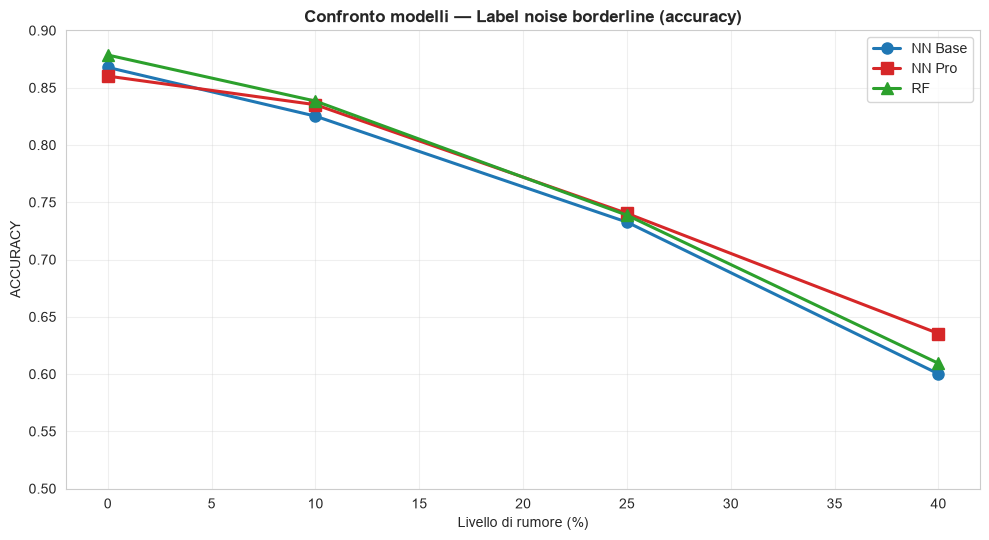
\includegraphics[width=0.86\textwidth]{lnb_compare_acc}\\[8pt]
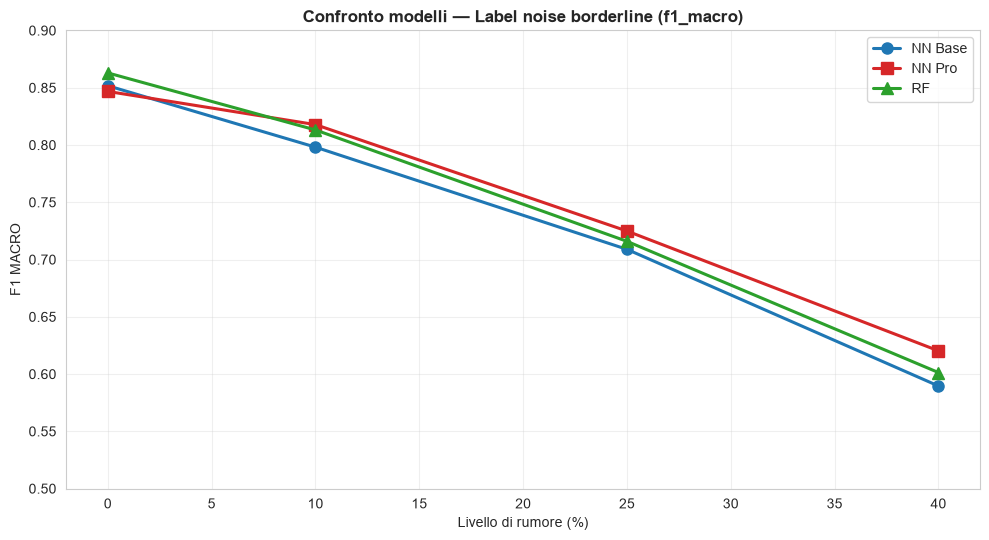
\includegraphics[width=0.86\textwidth]{lnb_compare_f1}
\caption{Label noise borderline: al 40\% tutti i modelli convergono attorno al 60\%, indicando il collasso predittivo.}
\label{fig:lnb_acc}
\end{figure}

A parità di intensità numerica rispetto all'alterazione stocastica, 
l'intervento borderline possiede una letalità geometrica intrinseca maggiore. 
L'inversione sistematica delle istanze vicine all'equatore spaziale che divide 
le classi induce lo spostamento macroscopico del confine decisionale. Le 
\textit{learning curves} della rete Pro (Figura~\ref{fig:lnb_curve}) non 
registrano alcun vantaggio apportato dalle regolarizzazioni né dagli arresti 
preventivi: di fronte a un'alterazione massiva della regione liminare di 
apprendimento, l'estrazione logica degli iperpiani non si dimostra 
recuperabile.

\begin{figure}[H]\centering
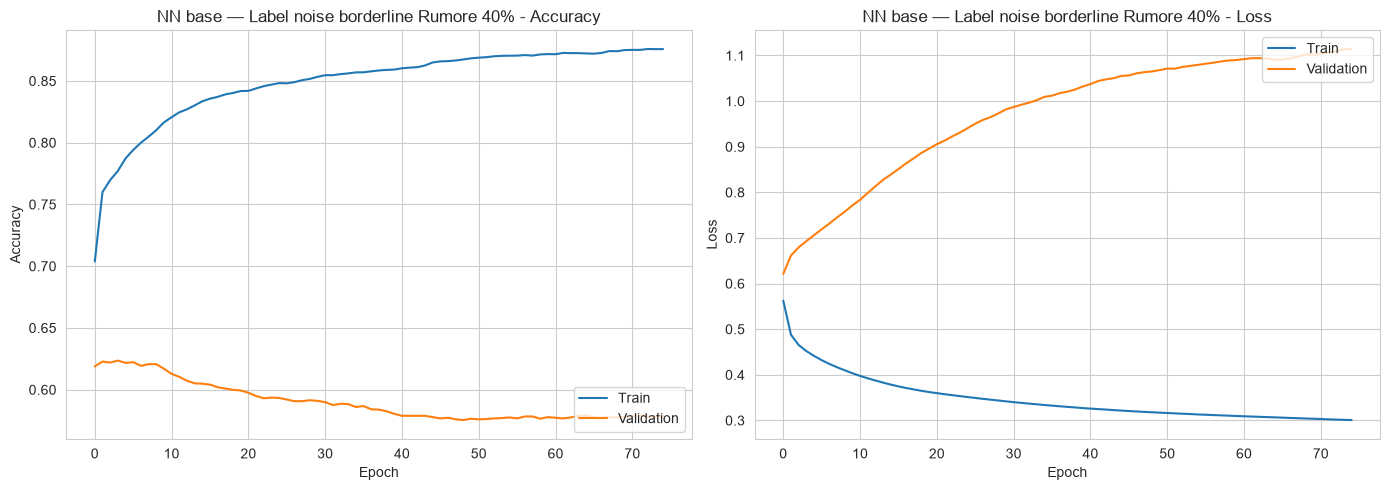
\includegraphics[width=0.9\textwidth]{lnb_nnbase_curve40}\\[8pt]
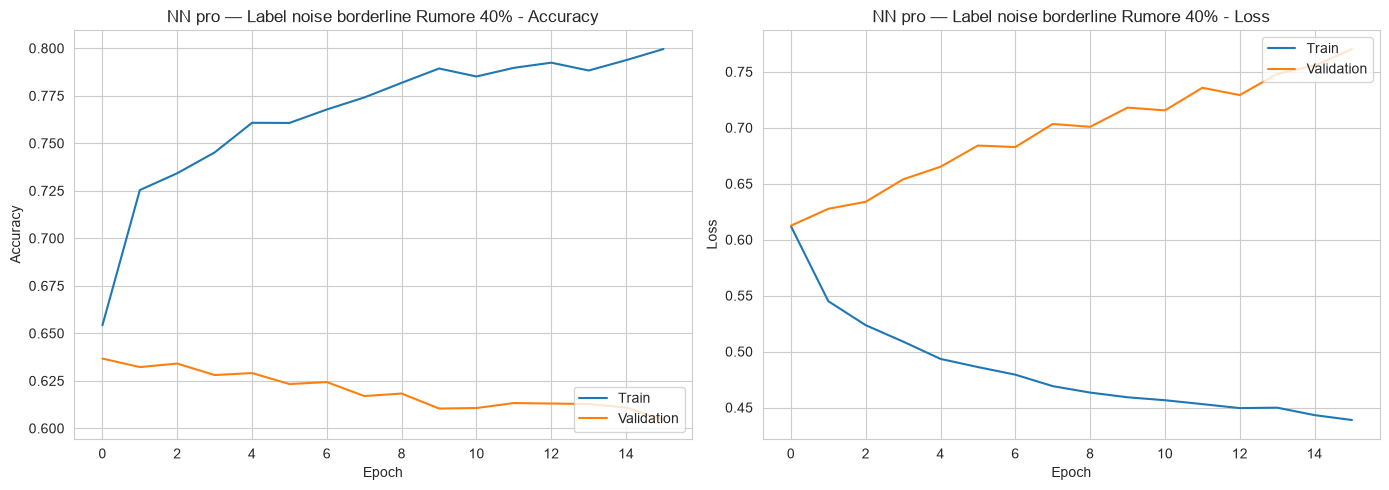
\includegraphics[width=0.9\textwidth]{lnb_nnpro_curve40}
\caption{Label noise borderline al 40\%: anche la validation della rete Pro crolla, a causa della falsificazione strutturale del confine decisionale.}
\label{fig:lnb_curve}
\end{figure}

A differenza delle fluttuazioni riscontrate sulle feature in continuo, il danno
inflitto alla classificazione si distribuisce in questo scenario in modo
sostanzialmente bilanciato tra le due classi: pur essendo i flip iniettati più
numerosi sulla classe maggioritaria (gamma), l'effetto sul test comporta un
incremento delle predizioni spurie su entrambe le variabili fisiche analizzate
(Figura~\ref{fig:lnb_cm}).

\begin{figure}[H]\centering
\begin{minipage}{0.49\textwidth}\centering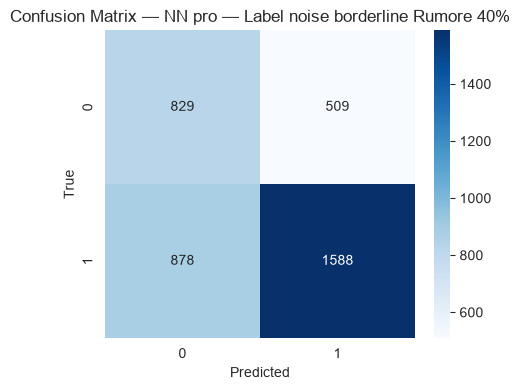
\includegraphics[width=\textwidth]{lnb_nnpro_cm40}\end{minipage}\hfill
\begin{minipage}{0.49\textwidth}\centering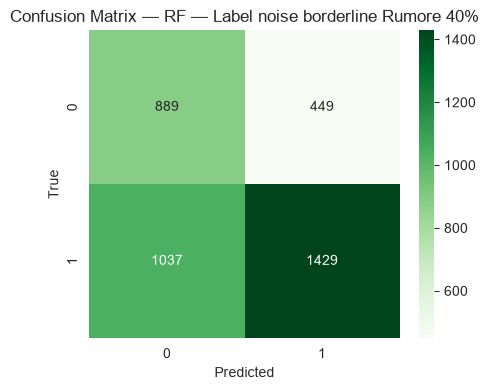
\includegraphics[width=\textwidth]{lnb_rf_cm40}\end{minipage}
\caption{Label noise borderline al 40\%: matrici di confusione della rete Pro (sinistra) e del Random Forest (destra). Errori diffusi in modo simmetrico.}
\label{fig:lnb_cm}
\end{figure}

% ---------- 9.4 Missing values ----------
\subsection{Missing values}

La sostituzione iterativa di singoli attributi con il valore nullo determina 
peggioramenti lineari e proporzionali a patto dell'inclusione logica di tecniche 
di ripristino. Sfruttando la mediana (variante definita canonica), 
le metriche globali conservano la fascia $82\%$--$85\%$ (Tabella~\ref{tab:mv}). 
In questa particolare casistica, l'algoritmo Random Forest assicura il minor 
cedimento, registrando un picco di accuratezza pari a $0{,}8528$ 
(Figura~\ref{fig:mv_acc}).

\begin{table}[H]\centering\footnotesize
\caption{Missing values (imputazione con mediana): metriche al variare del tasso di valori mancanti.}\label{tab:mv}
\begin{tabular}{c *{9}{c}}
\toprule
 & \multicolumn{3}{c}{NN Base} & \multicolumn{3}{c}{NN Pro} & \multicolumn{3}{c}{Random Forest}\\
\cmidrule(lr){2-4}\cmidrule(lr){5-7}\cmidrule(lr){8-10}
Rumore & Acc & F1$_m$ & AUC & Acc & F1$_m$ & AUC & Acc & F1$_m$ & AUC \\
\midrule
Pulito & 0.8678 & 0.85 & 0.9214 & 0.8601 & 0.85 & 0.9238 & 0.8785 & 0.86 & 0.9300 \\
10\% & 0.8423 & 0.82 & 0.8947 & 0.8375 & 0.82 & 0.9002 & 0.8559 & 0.84 & 0.9051 \\
25\% & 0.8123 & 0.79 & 0.8645 & 0.7978 & 0.78 & 0.8649 & 0.8270 & 0.80 & 0.8750 \\
40\% & 0.7792 & 0.74 & 0.8266 & 0.7650 & 0.75 & 0.8319 & 0.8068 & 0.78 & 0.8477 \\
\bottomrule
\end{tabular}
\end{table}


\begin{figure}[H]\centering
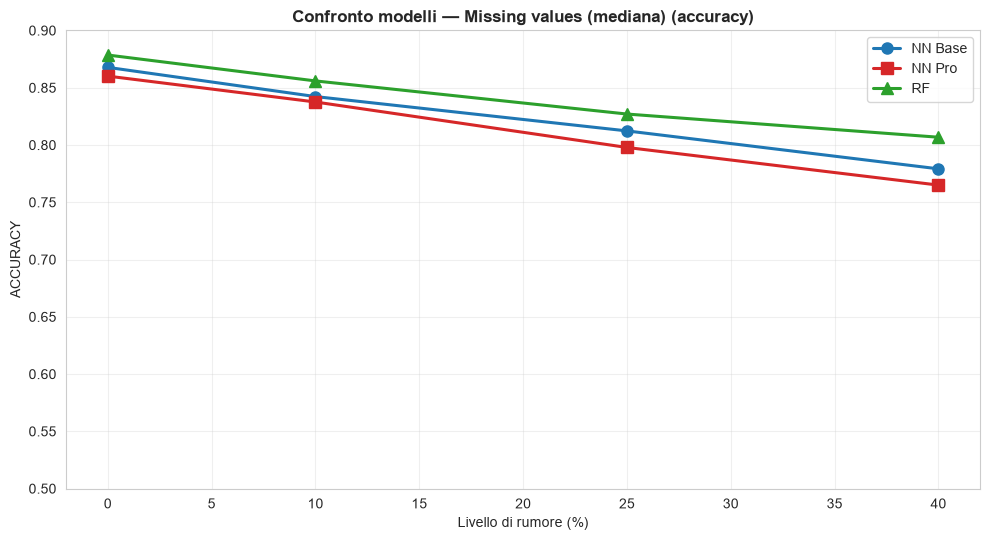
\includegraphics[width=0.86\textwidth]{mv_compare_acc}\\[8pt]
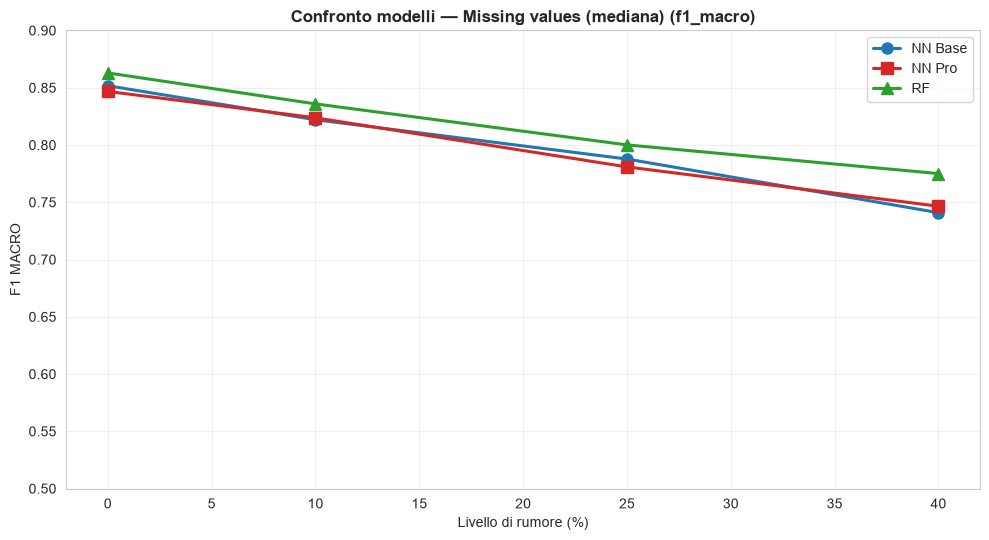
\includegraphics[width=0.86\textwidth]{mv_compare_f1}
\caption{Missing values con imputazione mediana. Il Random Forest mantiene un vantaggio costante a tutti i livelli.}
\label{fig:mv_acc}
\end{figure}

Il paragone strumentale tra l'impiego della media e l'impiego della mediana
(Figura~\ref{fig:mv_strat}) ridimensiona tuttavia le aspettative riposte nello
studio sulle asimmetrie distributive: il divario tra le due strategie resta
marginale e privo di una direzione univoca. Indifferente ai campioni posizionati
sulle code lunghe, la mediana acquisisce un lieve vantaggio soltanto sulla rete
Base ai livelli di corruzione più elevati; sulla rete Pro è invece la media a
risultare leggermente preferibile, mentre sul Random Forest le due imputazioni
si equivalgono. La mediana viene mantenuta come riferimento canonico per la sua
maggiore robustezza teorica alle code, ma sul piano empirico la scelta tra le due
strategie incide in misura trascurabile sulle prestazioni finali. Nel contesto
strutturale, l'algoritmo a foresta isola con maggiore flessibilità le istanze
falsificate in quanto i suoi operatori si basano su divisioni del campione e non
su pesi distribuiti lungo flussi di nodi.

\begin{figure}[H]\centering
\begin{minipage}{0.32\textwidth}\centering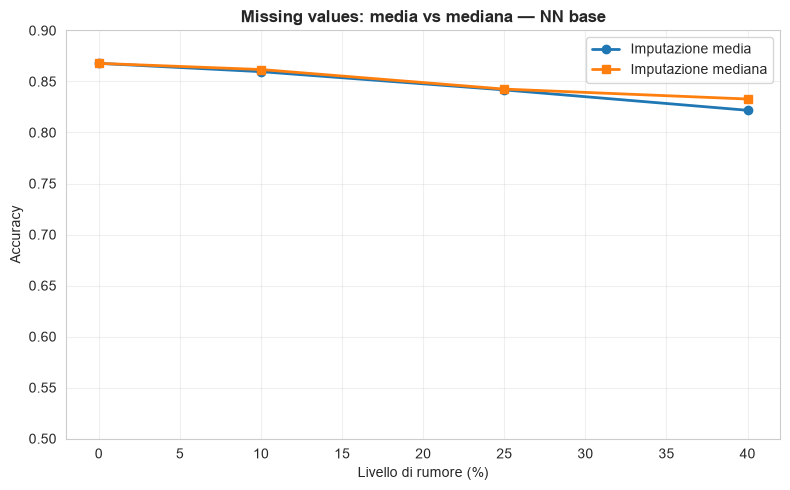
\includegraphics[width=\textwidth]{mv_meanmedian_nnbase}\end{minipage}\hfill
\begin{minipage}{0.32\textwidth}\centering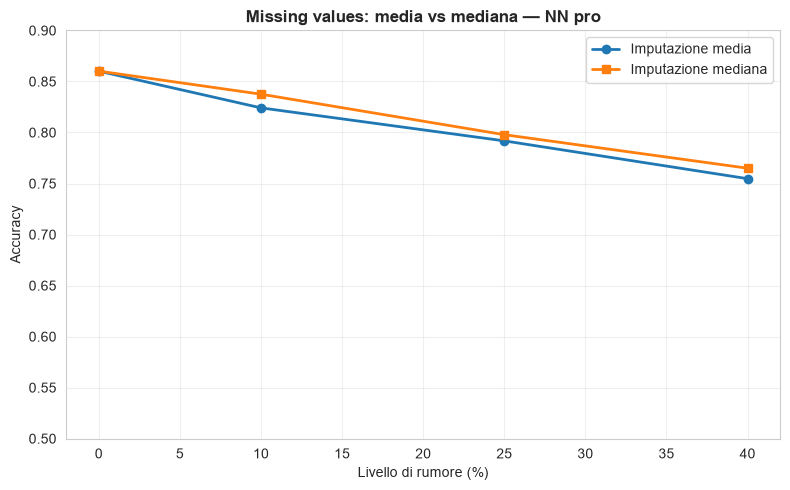
\includegraphics[width=\textwidth]{mv_meanmedian_nnpro}\end{minipage}\hfill
\begin{minipage}{0.32\textwidth}\centering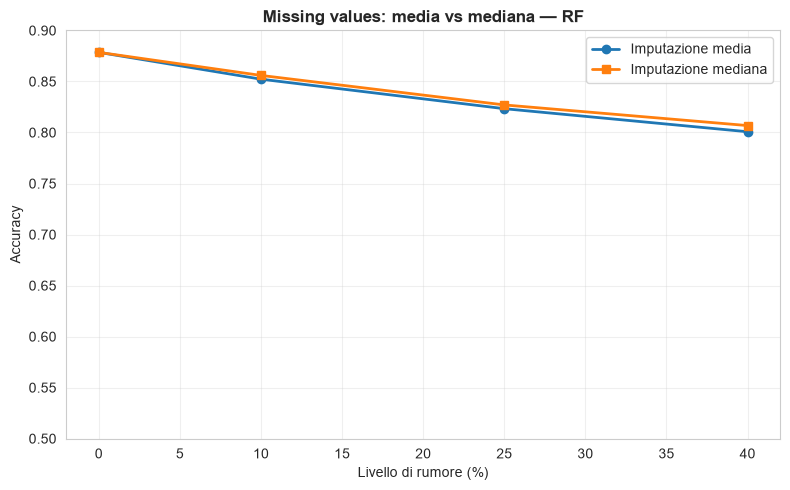
\includegraphics[width=\textwidth]{mv_meanmedian_rf}\end{minipage}
\caption{Missing values: confronto tra imputazione con media e con mediana per i tre modelli. Le due strategie producono prestazioni pressoché equivalenti; la mediana prevale lievemente solo sulla rete Base ad alta corruzione, mentre sulla rete Pro è la media a risultare marginalmente migliore.}
\label{fig:mv_strat}
\end{figure}

\begin{figure}[H]\centering
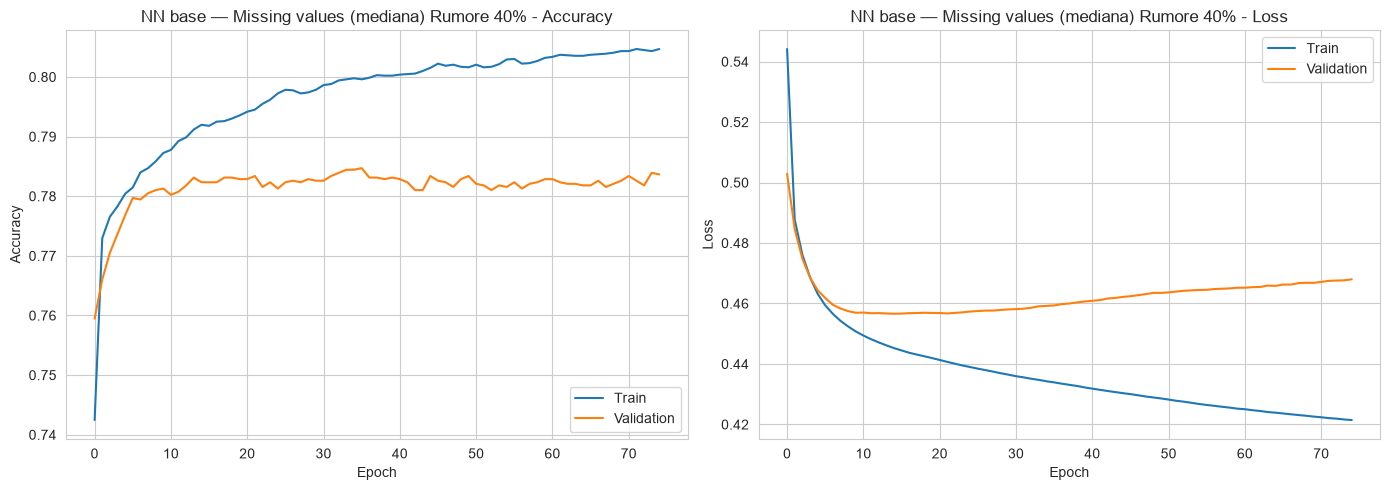
\includegraphics[width=0.9\textwidth]{mv_nnbase_curve40}\\[8pt]
\begin{minipage}{0.49\textwidth}\centering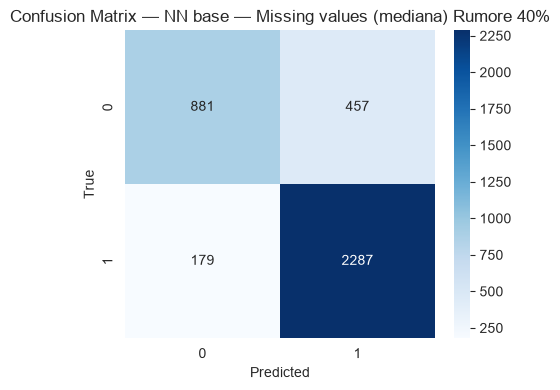
\includegraphics[width=\textwidth]{mv_nnbase_cm40}\end{minipage}\hfill
\begin{minipage}{0.49\textwidth}\centering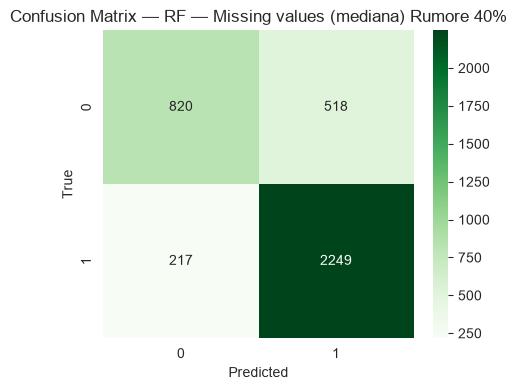
\includegraphics[width=\textwidth]{mv_rf_cm40}\end{minipage}
\caption{Missing values (mediana) al 40\%: curve della rete Base e matrici di confusione. L'addestramento è regolare; gli errori pesano sugli adroni.}
\label{fig:mv_cm}
\end{figure}

% ---------- 9.5 Outlier ----------
\subsection{Outlier}

A dispetto delle proiezioni preliminari, le infiltrazioni di valori massimali
estranei configurano l'anomalia di minore impatto sul comportamento diagnostico
(Tabella~\ref{tab:out}). L'accuratezza staziona attorno alla quota originaria
dell'$85\%$--$87\%$, non delineando significative tendenze degradative
(Figura~\ref{fig:out_acc}). La ragione di fondo non risiede tanto nel
trattamento applicato quanto nella natura stessa del disturbo: le righe
corrotte assumono valori a $\pm 5$ deviazioni standard con segno casuale e
del tutto scorrelato dall'etichetta, per cui il loro contributo al gradiente si
media verso lo zero e i modelli, addestrati su un test set pulito, ne risentono
poco.

\begin{table}[H]\centering\footnotesize
\caption{Outlier (winsorizzazione): metriche al variare della frazione di campioni anomali.}\label{tab:out}
\begin{tabular}{c *{9}{c}}
\toprule
 & \multicolumn{3}{c}{NN Base} & \multicolumn{3}{c}{NN Pro} & \multicolumn{3}{c}{Random Forest}\\
\cmidrule(lr){2-4}\cmidrule(lr){5-7}\cmidrule(lr){8-10}
Rumore & Acc & F1$_m$ & AUC & Acc & F1$_m$ & AUC & Acc & F1$_m$ & AUC \\
\midrule
Pulito & 0.8678 & 0.85 & 0.9214 & 0.8601 & 0.85 & 0.9238 & 0.8785 & 0.86 & 0.9300 \\
10\% & 0.8657 & 0.85 & 0.9196 & 0.8583 & 0.84 & 0.9220 & 0.8788 & 0.86 & 0.9295 \\
25\% & 0.8628 & 0.84 & 0.9160 & 0.8441 & 0.83 & 0.9173 & 0.8751 & 0.86 & 0.9267 \\
40\% & 0.8615 & 0.84 & 0.9116 & 0.8541 & 0.84 & 0.9201 & 0.8736 & 0.86 & 0.9250 \\
\bottomrule
\end{tabular}
\end{table}


\begin{figure}[H]\centering
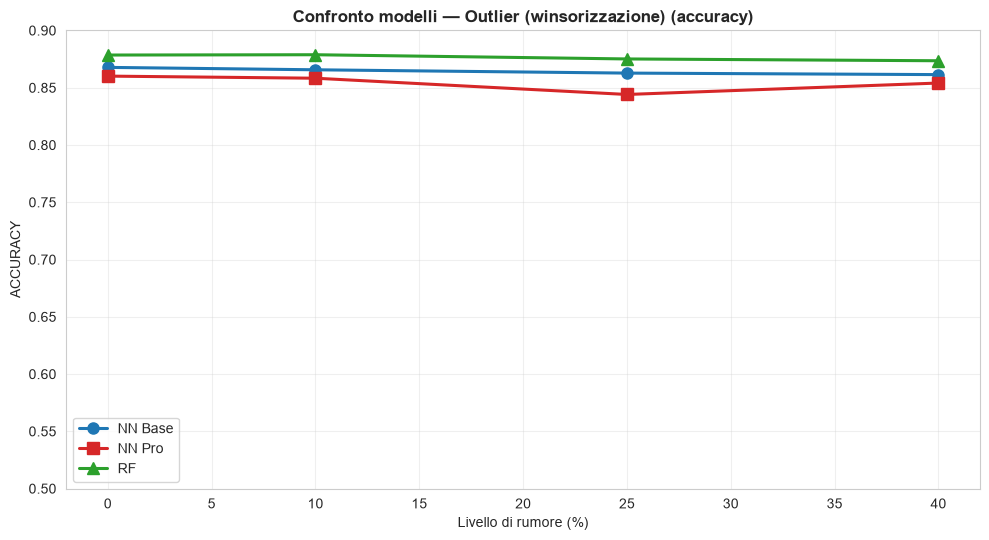
\includegraphics[width=0.86\textwidth]{out_compare_acc}\\[8pt]
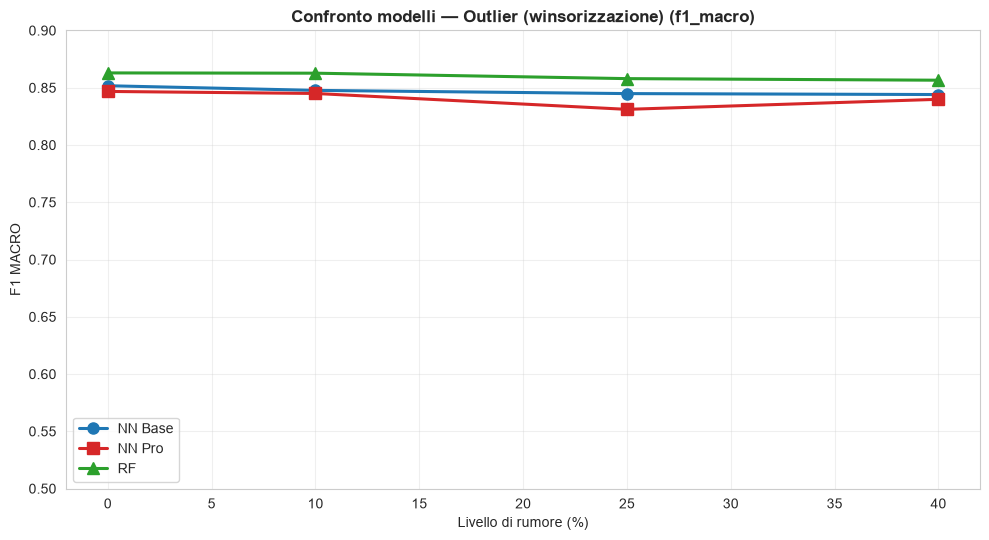
\includegraphics[width=0.86\textwidth]{out_compare_f1}
\caption{Outlier con winsorizzazione. Curve prestazionali pressoché inalterate.}
\label{fig:out_acc}
\end{figure}

Le disparità originate dai tre approcci in competizione
(Figura~\ref{fig:out_strat}) rimangono esigue: lasciare gli outlier inalterati,
winsorizzare o imputare produce risultati pressoché sovrapponibili. Questa
equivalenza conferma che, a tassi di corruzione elevati, la winsorizzazione al
$5\%$ è in larga parte inefficace — quando una frazione consistente di valori è
collassata su $\pm 5$, i percentili stessi risultano saturati e il troncamento
non rimuove gli estremi — e che la robustezza osservata va attribuita
all'intrinseca innocuità del disturbo più che alla strategia di mitigazione. La
winsorizzazione viene comunque mantenuta come variante canonica per prudenza, in
quanto assetto precauzionale ragionevole senza controindicazioni
(Figura~\ref{fig:out_cm}).

\begin{figure}[H]\centering
\begin{minipage}{0.32\textwidth}\centering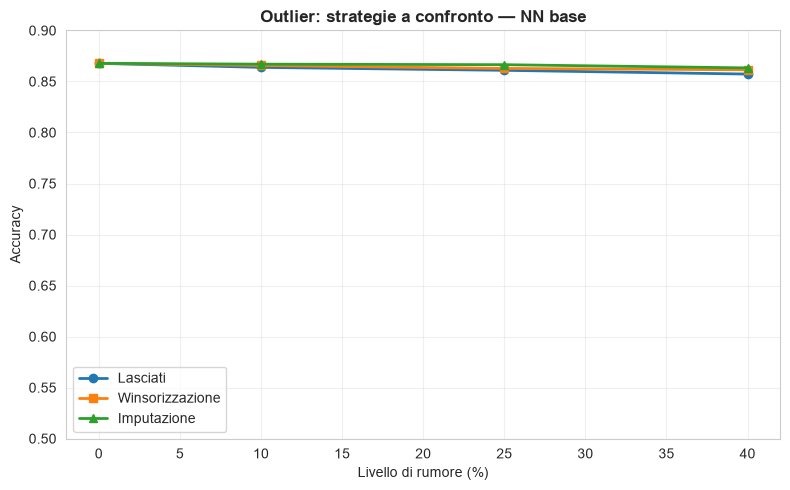
\includegraphics[width=\textwidth]{out_strategies_nnbase}\end{minipage}\hfill
\begin{minipage}{0.32\textwidth}\centering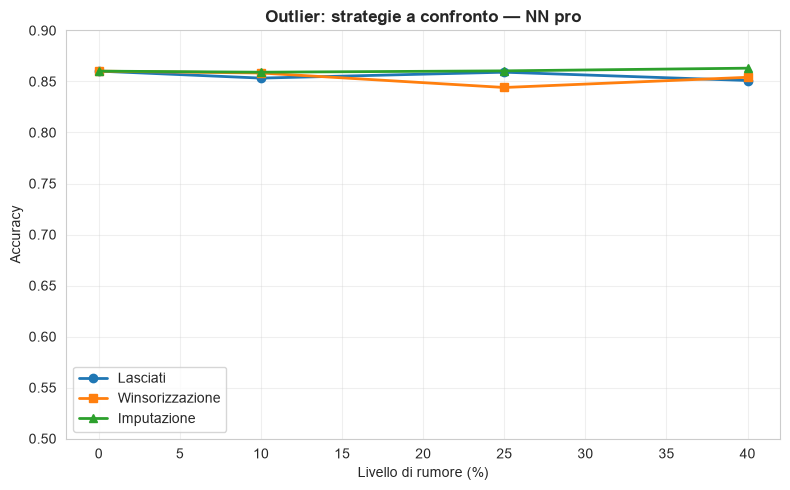
\includegraphics[width=\textwidth]{out_strategies_nnpro}\end{minipage}\hfill
\begin{minipage}{0.32\textwidth}\centering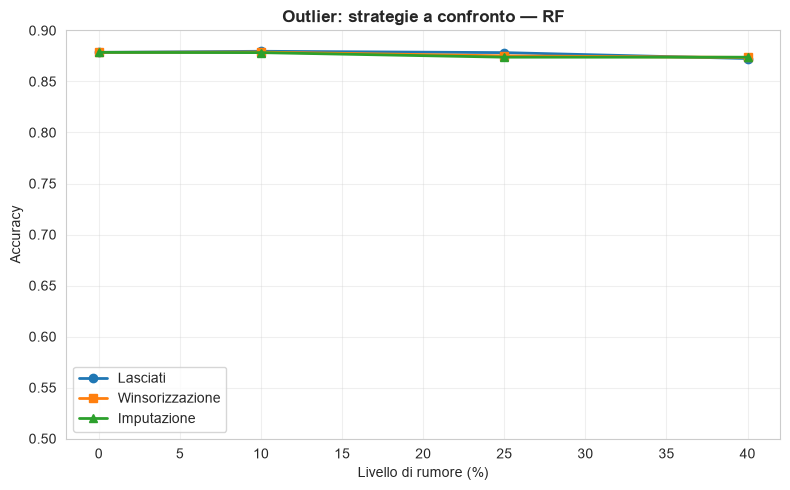
\includegraphics[width=\textwidth]{out_strategies_rf}\end{minipage}
\caption{Outlier: confronto tra le strategie. Le differenze sono minimali, supportate in buona parte dal preprocessing di standardizzazione.}
\label{fig:out_strat}
\end{figure}

\begin{figure}[H]\centering
\begin{minipage}{0.49\textwidth}\centering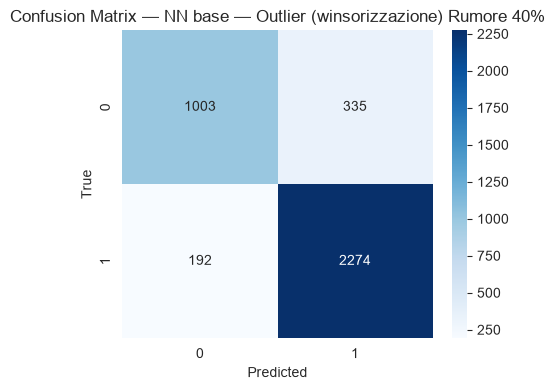
\includegraphics[width=\textwidth]{out_nnbase_cm40}\end{minipage}\hfill
\begin{minipage}{0.49\textwidth}\centering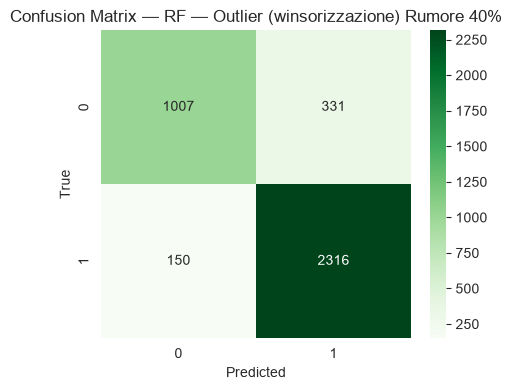
\includegraphics[width=\textwidth]{out_rf_cm40}\end{minipage}
\caption{Outlier (winsorizzazione) al 40\%: matrici di confusione. Prestazioni indistinguibili dal caso pulito.}
\label{fig:out_cm}
\end{figure}

% ---------- 9.6 Missing feature ----------
\subsection{Missing feature (sensore guasto)}

Il blocco iterativo delle acquisizioni strutturali del telescopio restituisce, 
parimenti al label noise, esiti catastrofici in virtù della privazione totale e 
incondizionata dei punti di riferimento spaziale. Estromettendo le informazioni 
generate dal canale \texttt{fAlpha} (Tabella~\ref{tab:mf}), si registra una 
caduta immediata di 4 o 5 punti netti; arrivando a coprire la cinquina maggiore, 
tutte le piattaforme testate franano sulla linea di confidenza marginale tra il 
$70\%$ e il $74\%$ (Figura~\ref{fig:mf_acc}).

\begin{table}[H]\centering\footnotesize
\caption{Missing feature: metriche rimuovendo le feature piu\' importanti (10\%$\to$top-1, 25\%$\to$top-3, 40\%$\to$top-5).}\label{tab:mf}
\begin{tabular}{c *{9}{c}}
\toprule
 & \multicolumn{3}{c}{NN Base} & \multicolumn{3}{c}{NN Pro} & \multicolumn{3}{c}{Random Forest}\\
\cmidrule(lr){2-4}\cmidrule(lr){5-7}\cmidrule(lr){8-10}
Rumore & Acc & F1$_m$ & AUC & Acc & F1$_m$ & AUC & Acc & F1$_m$ & AUC \\
\midrule
Pulito & 0.8678 & 0.85 & 0.9214 & 0.8601 & 0.85 & 0.9238 & 0.8785 & 0.86 & 0.9300 \\
10\% & 0.8215 & 0.79 & 0.8675 & 0.8052 & 0.79 & 0.8716 & 0.8294 & 0.80 & 0.8788 \\
25\% & 0.7773 & 0.74 & 0.8007 & 0.7574 & 0.73 & 0.7991 & 0.7836 & 0.75 & 0.8195 \\
40\% & 0.7303 & 0.67 & 0.7413 & 0.6995 & 0.67 & 0.7347 & 0.7363 & 0.68 & 0.7494 \\
\bottomrule
\end{tabular}
\end{table}


\begin{figure}[H]\centering
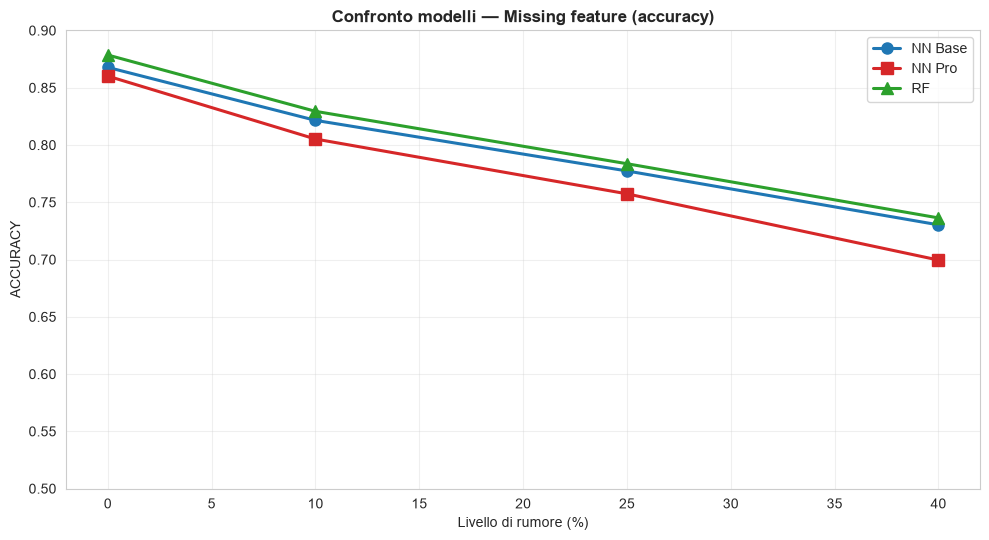
\includegraphics[width=0.86\textwidth]{mf_compare_acc}\\[8pt]
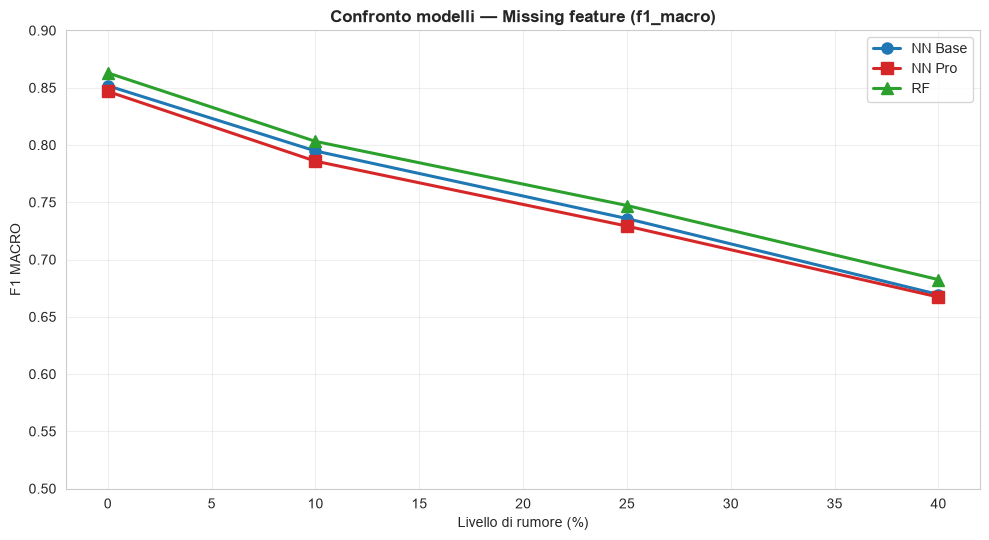
\includegraphics[width=0.86\textwidth]{mf_compare_f1}
\caption{Missing feature: accuratezza (in alto) e F1 macro (in basso). Rimuovere \texttt{fAlpha} genera il declino più severo registrato fin dalla prima istanza.}
\label{fig:mf_acc}
\end{figure}

Quest'ultima simulazione rimarca l'effettivo coefficiente di importanza detenuto 
dal vettore diagnostico \texttt{fAlpha}. A fronte della scarsissima affiliazione 
di correlazione stabilita con le altre componenti in analisi, il suo decadimento 
comporta un depauperamento insostituibile. In controtendenza allo scenario con 
rumore, la totale assenza di nozioni informative paralizza le routine di 
regolarizzazione, spingendo la rete neurale Pro in coda al gruppo valutativo 
($0{,}6995$ al $40\%$), in virtù delle rigidità intrinseche ai meccanismi di 
profilassi dall'overfitting. L'asportazione chirurgica dei dati compromette 
prioritariamente i canali minoritari, annientando il potere di deduzione della 
categoria adroni (Figura~\ref{fig:mf_cm} e \ref{fig:mf_progress}).

\begin{figure}[H]\centering
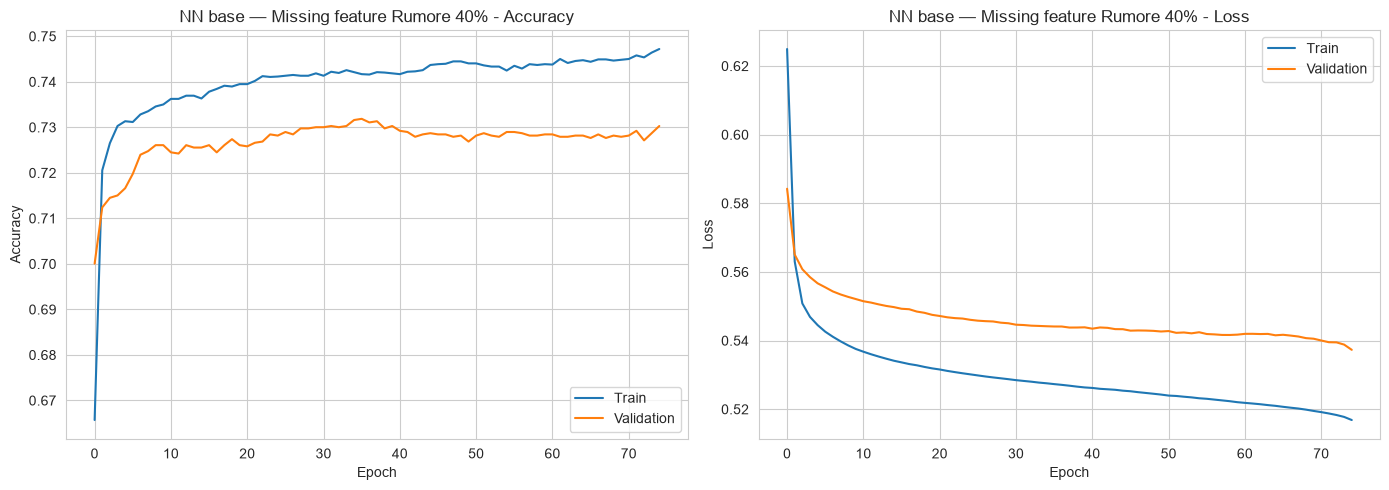
\includegraphics[width=0.9\textwidth]{mf_nnbase_curve40}\\[8pt]
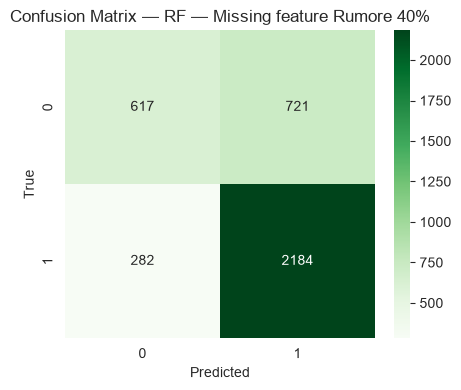
\includegraphics[width=0.5\textwidth]{mf_rf_cm40}
\caption{Missing feature al 40\%. Senza le feature più informative i modelli perdono potere discriminante intrinseco, pur mantenendo learning curves stabili e vicine.}
\label{fig:mf_cm}
\end{figure}

\begin{figure}[H]\centering
\begin{minipage}{0.32\textwidth}\centering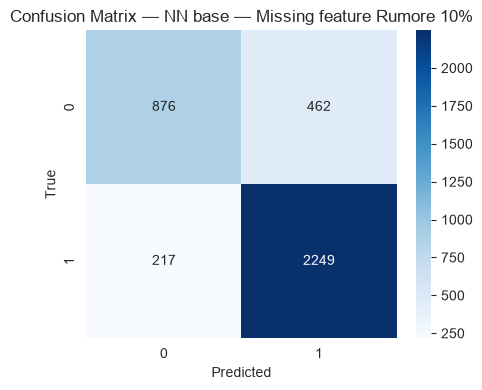
\includegraphics[width=\textwidth]{mf_nnbase_cm10}\end{minipage}\hfill
\begin{minipage}{0.32\textwidth}\centering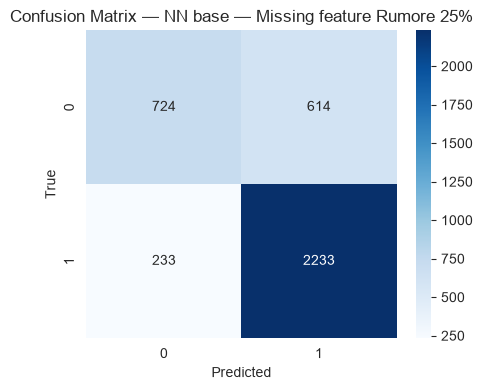
\includegraphics[width=\textwidth]{mf_nnbase_cm25}\end{minipage}\hfill
\begin{minipage}{0.32\textwidth}\centering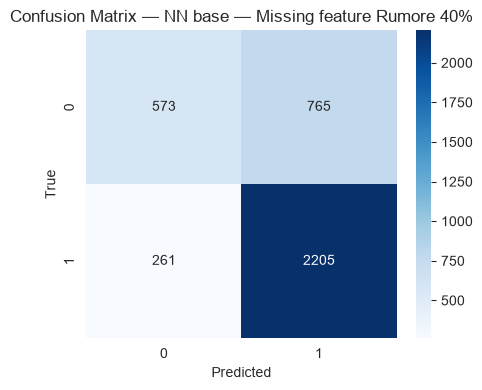
\includegraphics[width=\textwidth]{mf_nnbase_cm40}\end{minipage}
\caption{Missing feature, rete Base: matrici di confusione. Rimuovendo le feature, la capacità di discriminazione sugli adroni svanisce progressivamente.}
\label{fig:mf_progress}
\end{figure}

% ============================================================
% 10. SINTESI TRASVERSALE
% ============================================================
\section{Sintesi trasversale}\label{sec:sintesi}

Una volta delineato il comportamento nei singoli scenari, l'analisi congiunta 
(Figura~\ref{fig:aggr}) riassume graficamente, su un unico parametro di scala, 
i livelli di degrado subiti. Le oscillazioni tra accuratezza globale e 
ponderazioni F1 tratteggiano il profilo immunitario di ciascun classificatore.

\begin{figure}[H]\centering
\begin{minipage}{0.32\textwidth}\centering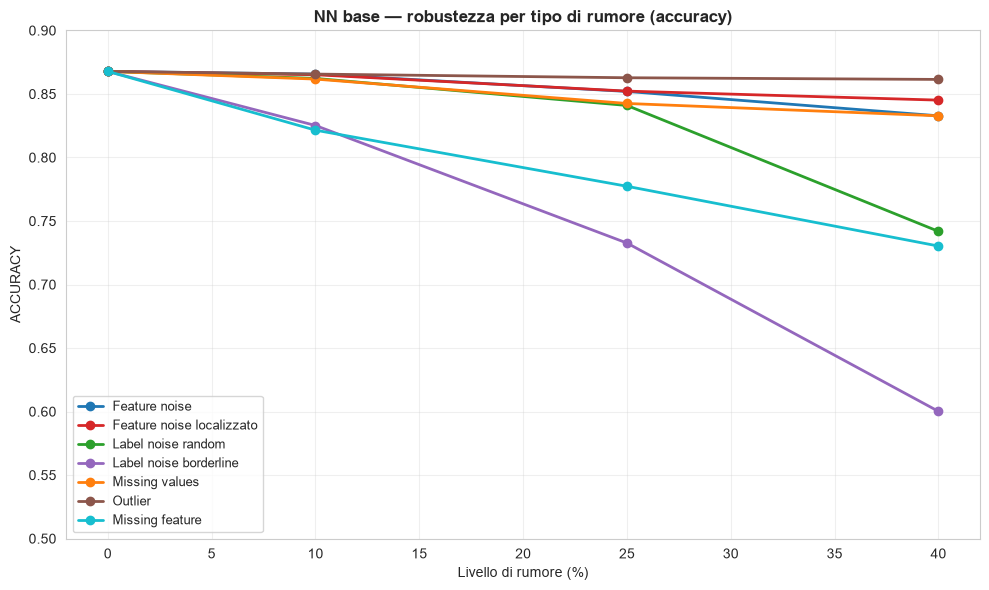
\includegraphics[width=\textwidth]{aggr_nnbase_acc}\end{minipage}\hfill
\begin{minipage}{0.32\textwidth}\centering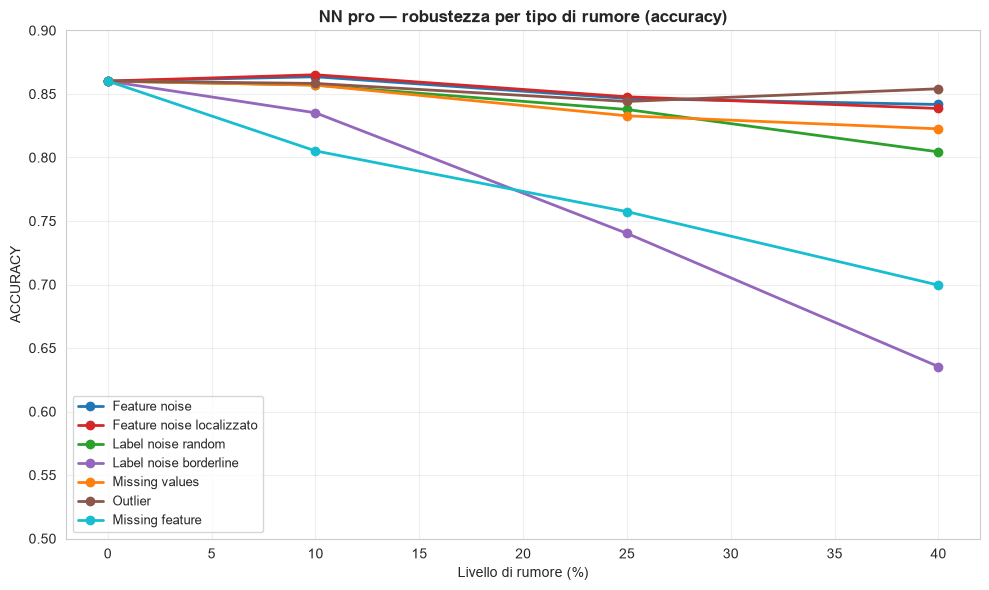
\includegraphics[width=\textwidth]{aggr_nnpro_acc}\end{minipage}\hfill
\begin{minipage}{0.32\textwidth}\centering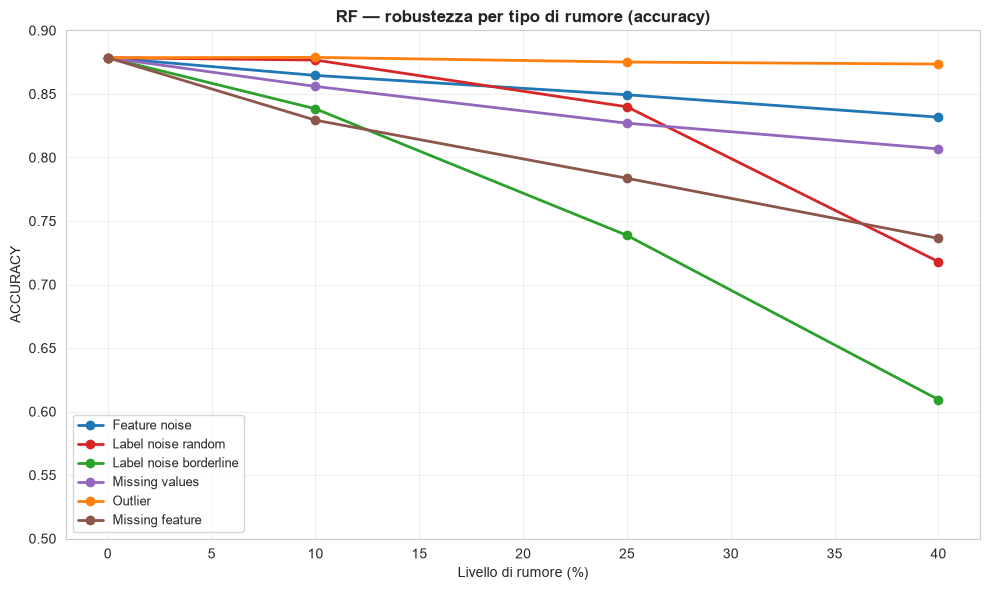
\includegraphics[width=\textwidth]{aggr_rf_acc}\end{minipage}\\[4pt]
\begin{minipage}{0.32\textwidth}\centering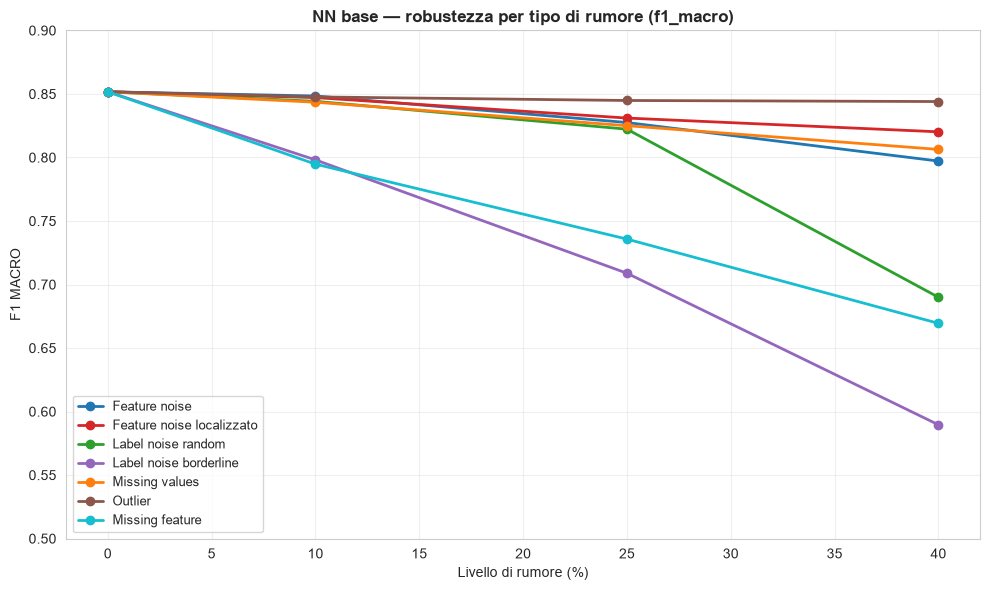
\includegraphics[width=\textwidth]{aggr_nnbase_f1}\end{minipage}\hfill
\begin{minipage}{0.32\textwidth}\centering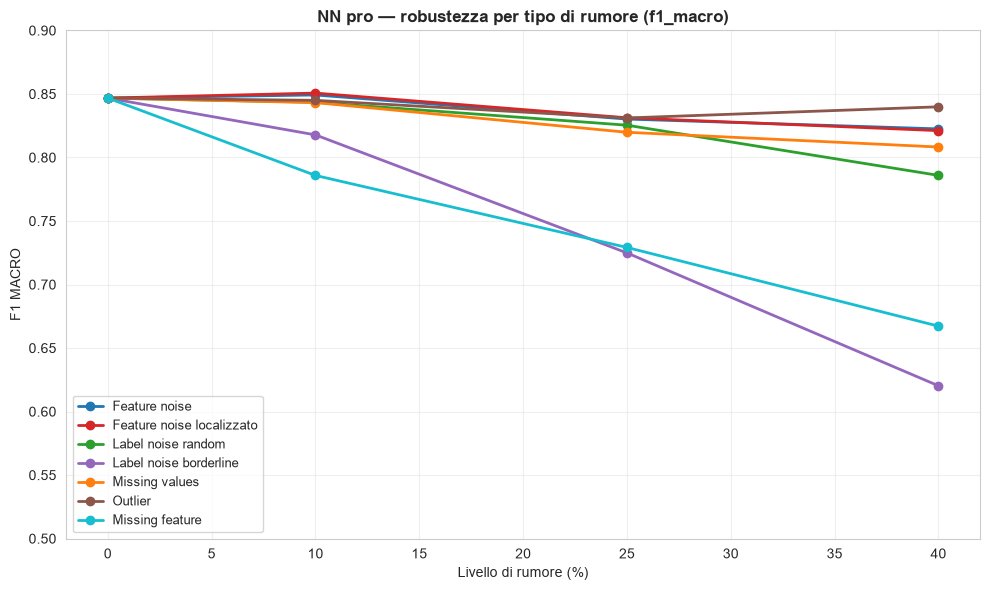
\includegraphics[width=\textwidth]{aggr_nnpro_f1}\end{minipage}\hfill
\begin{minipage}{0.32\textwidth}\centering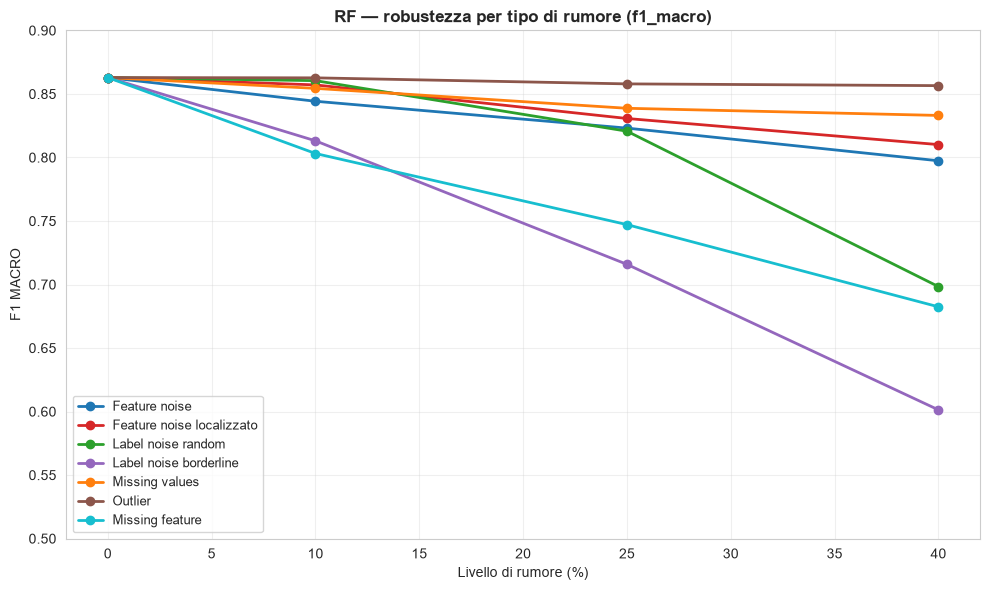
\includegraphics[width=\textwidth]{aggr_rf_f1}\end{minipage}
\caption{Robustezza per tipo di rumore. Emerge costantemente l'outlier come disturbo innocuo e il label noise borderline come criticità massima.}
\label{fig:aggr}
\end{figure}

L'evidenza stabilisce una gerarchia di vulnerabilità condivisa. Gli outlier si 
distinguono come i fattori meno disturbanti, affiancati a stretto raggio dal 
feature noise e dalle celle deficitarie, limitati da cali moderati e gestibili. 
Al capo diametralmente opposto, la variazione topologica delle classi di confine 
costituisce la perturbazione estrema, portando alla compromissione assoluta. La 
heatmap (Figura~\ref{fig:heatmap}) cristallizza questi trend nel picco negativo 
(40\% di corruzione), indicando cromaticamente l'annullamento della validità del 
labeling borderline rispetto al verde tenue delle proiezioni per outlier.

\begin{figure}[H]\centering
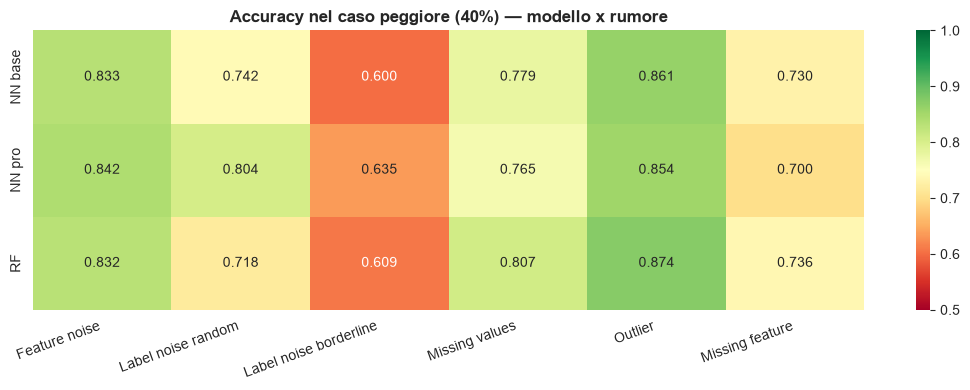
\includegraphics[width=0.98\textwidth]{summary_heatmap}
\caption{Accuratezza estrema nel caso peggiore (40\%) per ogni combinazione. Il rosso intenso sul label noise borderline indica l'annullamento dei gradienti logici.}
\label{fig:heatmap}
\end{figure}

In ottica di contenimento (Figura~\ref{fig:degr}), emerge innegabilmente la forte 
tolleranza ai mutamenti continui posseduta dalla rete regolarizzata (NN Pro), 
bilanciata tuttavia dalla sensibilità mostrata a fronte delle alterazioni ad 
impatto soppressivo, frangente in cui le foreste di alberi dominano su ogni 
scenario per flessibilità strutturale.

\begin{figure}[H]\centering
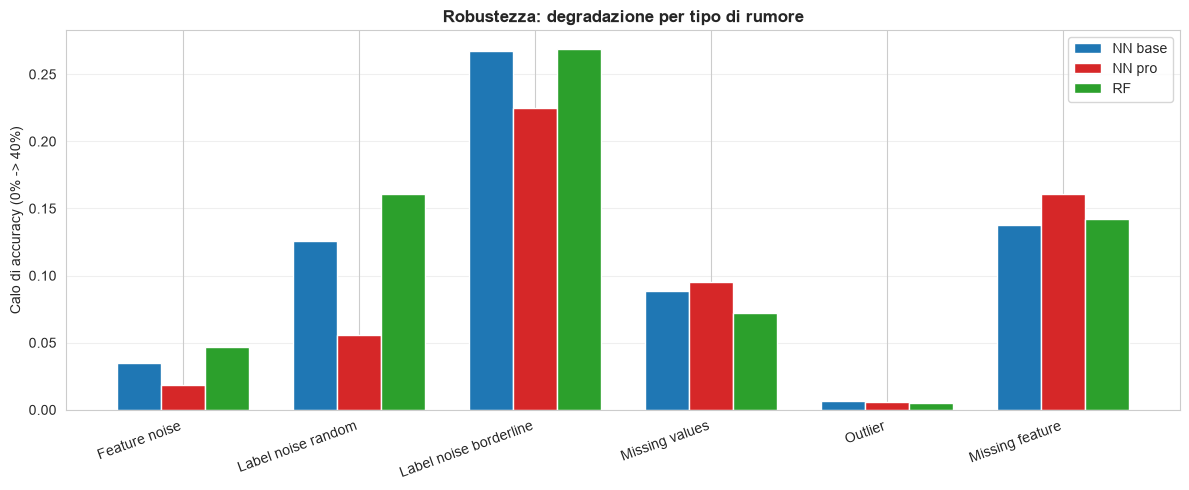
\includegraphics[width=0.98\textwidth]{summary_degradation}
\caption{Calo di accuratezza. Barre contenute indicano maggiore tenuta ai gradienti spuri e al data leakage.}
\label{fig:degr}
\end{figure}

Estrapolando una media complessiva (Figura~\ref{fig:rank}), le distanze globali si 
assottigliano fino alla sovrapposizione concettuale. Il vertice occupato dalla rete 
strutturata (0,785), e tallonato da Random Forest (0,780) e NN base (0,778), impone 
valutazioni contestuali alla messa in opera reale: la scelta non obbedisce al 
modello astratto, ma al background specifico da cui verranno generati gli input.

\begin{figure}[H]\centering
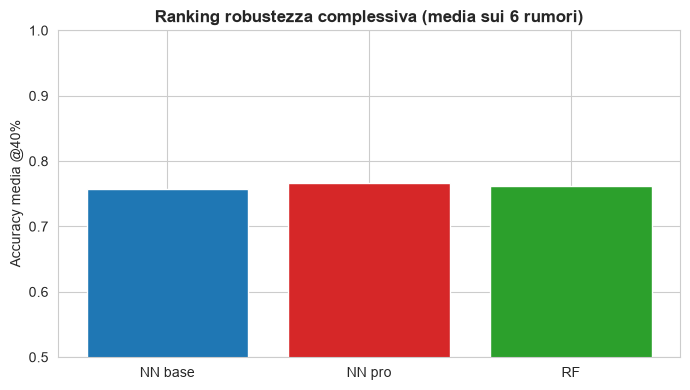
\includegraphics[width=0.74\textwidth]{summary_ranking}
\caption{Robustezza complessiva (accuratezza media). I tre modelli convergono in uno spazio di deviazione trascurabile.}
\label{fig:rank}
\end{figure}

La proiezione ROC incrociata sulla perturbazione gaussiana (Figura~\ref{fig:roc}) 
valida inoltre le capacità analitiche di ranking del test, assicurando che lo scarto 
si traduca essenzialmente in un incremento adattativo della rete naive (NN base) ed 
in un posizionamento coerente della controparte regolare.

\begin{figure}[H]\centering
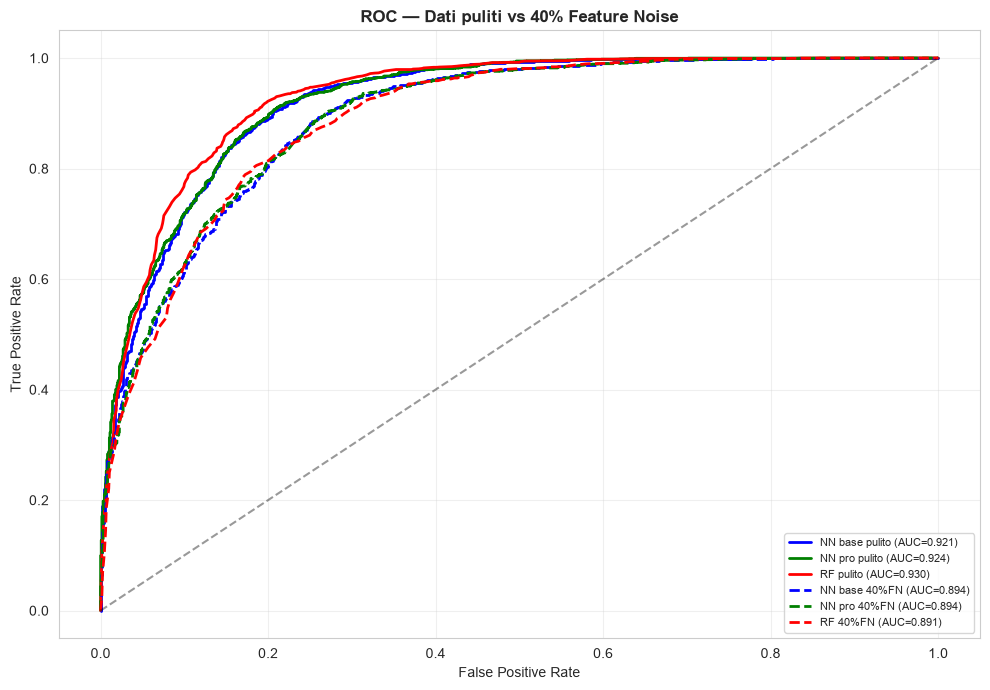
\includegraphics[width=0.90\textwidth]{roc_clean_vs_fn40}
\caption{Curve ROC dei tre modelli su dati puliti (continue) e con 40\% di feature noise (tratteggiate). Il feature noise erode limitatamente la classificazione ordinale.}
\label{fig:roc}
\end{figure}

\subsection{Controllo multi-seed}\label{sec:multiseed}

Tutti i risultati discussi finora derivano da un singolo seme casuale
(\texttt{seed = 42}). Per escludere che il degrado osservato sia un artefatto
dovuto a una particolare partizione dei dati o a una specifica inizializzazione
dei pesi, l'esperimento di \emph{feature noise} è stato ripetuto in modo
identico su cinque semi distinti $\{42, 7, 123, 2024, 99\}$. Ogni seme governa
contemporaneamente la realizzazione del rumore gaussiano, lo split
train/validation/test e l'inizializzazione dei tre modelli; per ciascun livello
di corruzione si riportano media e deviazione standard delle metriche
(Tabella~\ref{tab:multiseed}).

\begin{table}[H]\centering\footnotesize
\caption{Controllo multi-seed sul feature noise: media $\pm$ deviazione standard delle metriche sui cinque semi $\{42, 7, 123, 2024, 99\}$. Le deviazioni standard restano dell'ordine del millesimo, ampiamente inferiori al divario tra livelli di rumore.}\label{tab:multiseed}
\begin{tabular}{ll ccc}
\toprule
Modello & Rumore & Accuracy & F1$_m$ & AUC \\
\midrule
NN Base & Pulito & $0.8685 \pm 0.0027$ & $0.8514 \pm 0.0029$ & $0.9220 \pm 0.0015$ \\
        & 10\%   & $0.8672 \pm 0.0018$ & $0.8487 \pm 0.0025$ & $0.9198 \pm 0.0014$ \\
        & 25\%   & $0.8526 \pm 0.0020$ & $0.8270 \pm 0.0024$ & $0.9068 \pm 0.0016$ \\
        & 40\%   & $0.8342 \pm 0.0031$ & $0.7997 \pm 0.0040$ & $0.8924 \pm 0.0027$ \\
\midrule
NN Pro  & Pulito & $0.8638 \pm 0.0035$ & $0.8497 \pm 0.0032$ & $0.9241 \pm 0.0010$ \\
        & 10\%   & $0.8631 \pm 0.0036$ & $0.8479 \pm 0.0030$ & $0.9204 \pm 0.0012$ \\
        & 25\%   & $0.8464 \pm 0.0045$ & $0.8293 \pm 0.0036$ & $0.9056 \pm 0.0016$ \\
        & 40\%   & $0.8328 \pm 0.0068$ & $0.8130 \pm 0.0070$ & $0.8924 \pm 0.0012$ \\
\midrule
Random Forest & Pulito & $0.8800 \pm 0.0013$ & $0.8645 \pm 0.0014$ & $0.9308 \pm 0.0009$ \\
        & 10\%   & $0.8646 \pm 0.0024$ & $0.8442 \pm 0.0026$ & $0.9198 \pm 0.0015$ \\
        & 25\%   & $0.8492 \pm 0.0016$ & $0.8228 \pm 0.0016$ & $0.9042 \pm 0.0018$ \\
        & 40\%   & $0.8285 \pm 0.0037$ & $0.7934 \pm 0.0055$ & $0.8881 \pm 0.0028$ \\
\bottomrule
\end{tabular}
\end{table}


L'esito è netto: le deviazioni standard restano contenute nell'ordine del
millesimo per ogni combinazione modello--livello, con un valore massimo di
appena $0{,}0068$ (rete Pro al $40\%$). Questa dispersione è di un ordine di
grandezza inferiore al calo prodotto dal rumore — la sola NN Base perde circa
$3{,}4$ punti percentuali di accuratezza passando dai dati puliti al $40\%$ —,
il che dimostra che la traiettoria di decadimento è un segnale reale indotto dai
dati e non semplice varianza procedurale. Le barre d'errore nelle
Figure~\ref{fig:ms_acc} e \ref{fig:ms_f1}, appena percepibili attorno ai
marcatori, rendono visivamente questa stabilità: le curve dei tre modelli sono
nettamente separate dalla propria incertezza statistica a ogni livello.

\begin{figure}[H]\centering
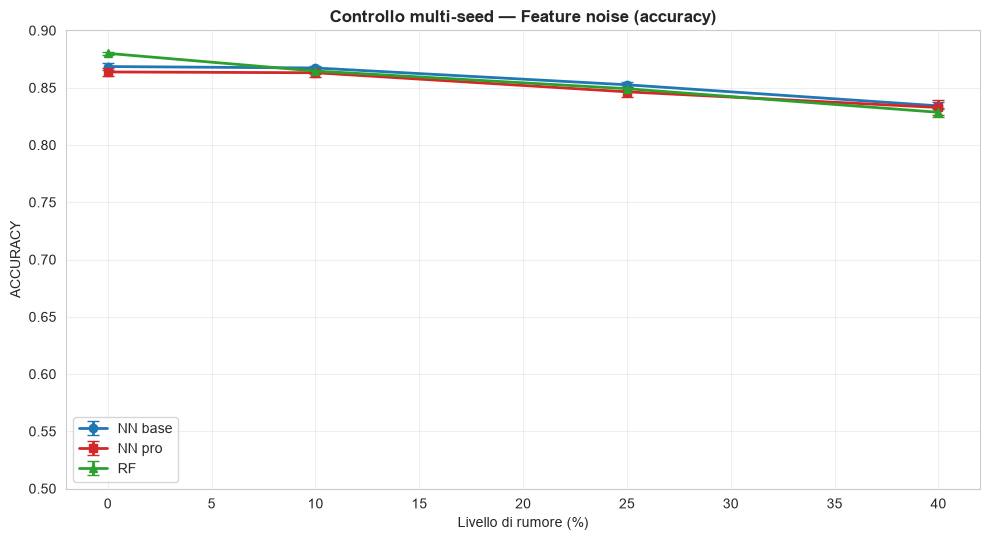
\includegraphics[width=0.82\textwidth]{ms_acc}
\caption{Controllo multi-seed (feature noise): accuratezza media sui cinque semi al variare del livello di rumore. Le barre d'errore ($\pm 1$ deviazione standard) sono quasi impercettibili, a conferma della riproducibilità del trend.}
\label{fig:ms_acc}
\end{figure}

\begin{figure}[H]\centering
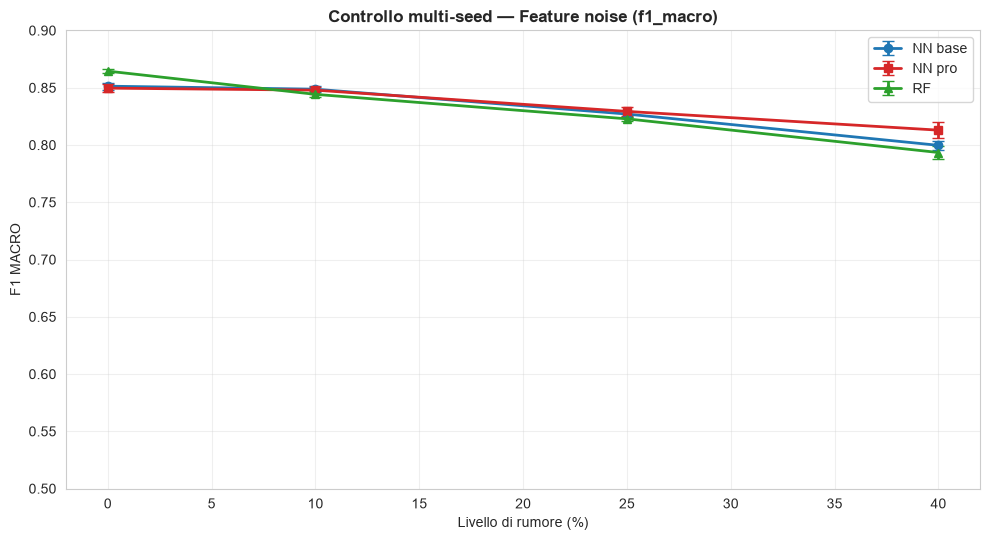
\includegraphics[width=0.82\textwidth]{ms_f1}
\caption{Controllo multi-seed (feature noise): F1 macro media sui cinque semi. Anche sulla metrica bilanciata l'ordinamento dei modelli e l'entità del degrado restano stabili tra i semi.}
\label{fig:ms_f1}
\end{figure}

La verifica conferma inoltre la gerarchia di robustezza emersa dall'analisi a
seme singolo: il Random Forest parte dal livello più alto sui dati puliti
($0{,}8800$) ma cede terreno più rapidamente, fino ad allinearsi alle reti
neurali al $40\%$; la rete Pro, grazie alla regolarizzazione, esibisce il
degrado più graduale pur partendo da una base leggermente inferiore. Tali
differenze, pienamente coerenti tra i cinque semi, escludono che l'ordinamento
osservato dipenda da fluttuazioni del generatore stocastico.

% ============================================================
% 11. PARTE NON SUPERVISIONATA
% ============================================================
\section{Analisi non supervisionata (K-Means)}\label{sec:kmeans}

Il ciclo valutativo ingloba un'ultima integrazione fondata sul raggruppamento in 
assenza di variabili dipendenti. Stabilito un raggio aggregativo pari a due 
conglomerati macroscopici, basato sull'interpolazione visiva dell'inerzia (metodo del
gomito) e sul valore della silhouette, massimo proprio in corrispondenza di $k=2$
(Figura~\ref{fig:kmeans_k}) — pur tenendo presente che la silhouette tende
strutturalmente a premiare valori di $k$ contenuti, per cui costituisce un
indizio più che una prova decisiva —
l'architettura conferma e restituisce riscontri duali ai precedenti
attestati supervisionati. L'anomalia sulle etichette risulta del tutto ininfluente ai fini 
dell'orientamento dei centroidi, in quanto i raggruppamenti geometrici nascono da un 
processo basato interamente sullo scarto euclideo, astraendo per necessità costruttive le 
impronte classificate in archivio.

\begin{figure}[H]\centering
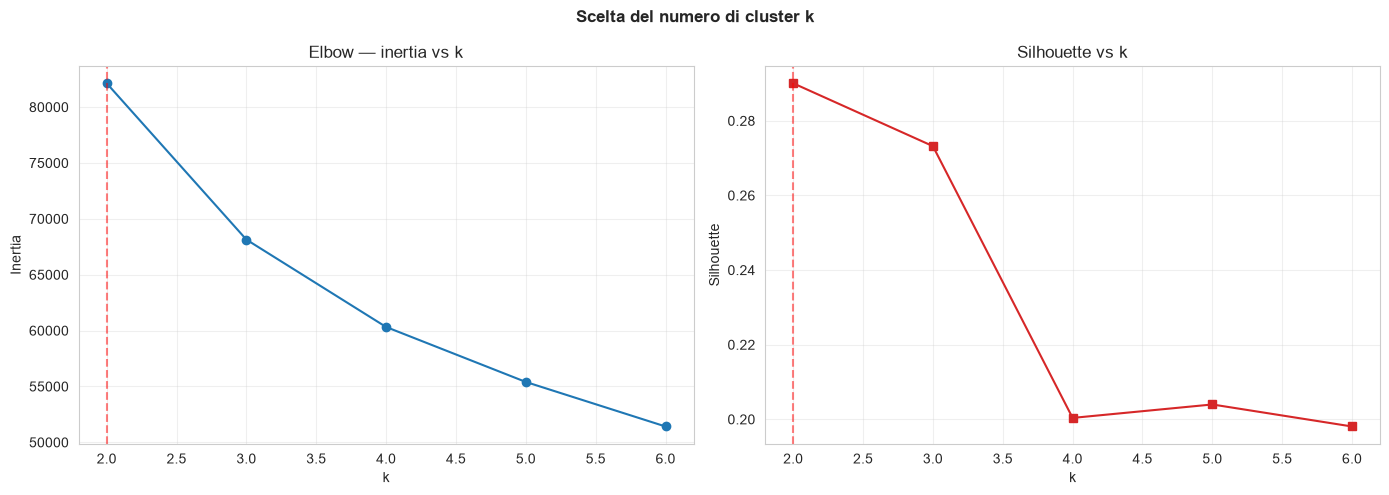
\includegraphics[width=0.92\textwidth]{kmeans_kselection}
\caption{Scelta del numero di cluster. Inerzia e silhouette indicano in $k=2$ la configurazione spaziale ottimale per la densità esplorata.}
\label{fig:kmeans_k}
\end{figure}

Le distanze geometriche generate falliscono nel mappare fedelmente i legami 
sostanziali tra sorgenti (adroniche contro fotoniche). L'assegnazione spaziale 
origina un valore Adjusted Rand Index pari a 0,006 (quasi nullo) accoppiato ad 
un indice di purezza equiparabile con lo scompenso probabilistico nativo dei dati. 
In sintesi, pur seguendo il profilo di varianza, l'algoritmo separa masse numeriche 
prive di connessione intima col fine di ricerca (Figura~\ref{fig:kmeans}). Le 
proprietà fisiche che demarcano i gruppi non risiedono sulla spaccatura dei pesi ma 
attraversano i conglomerati senza offrire discriminanti lineari o raggruppabili allo 
spazio.

\begin{figure}[H]\centering
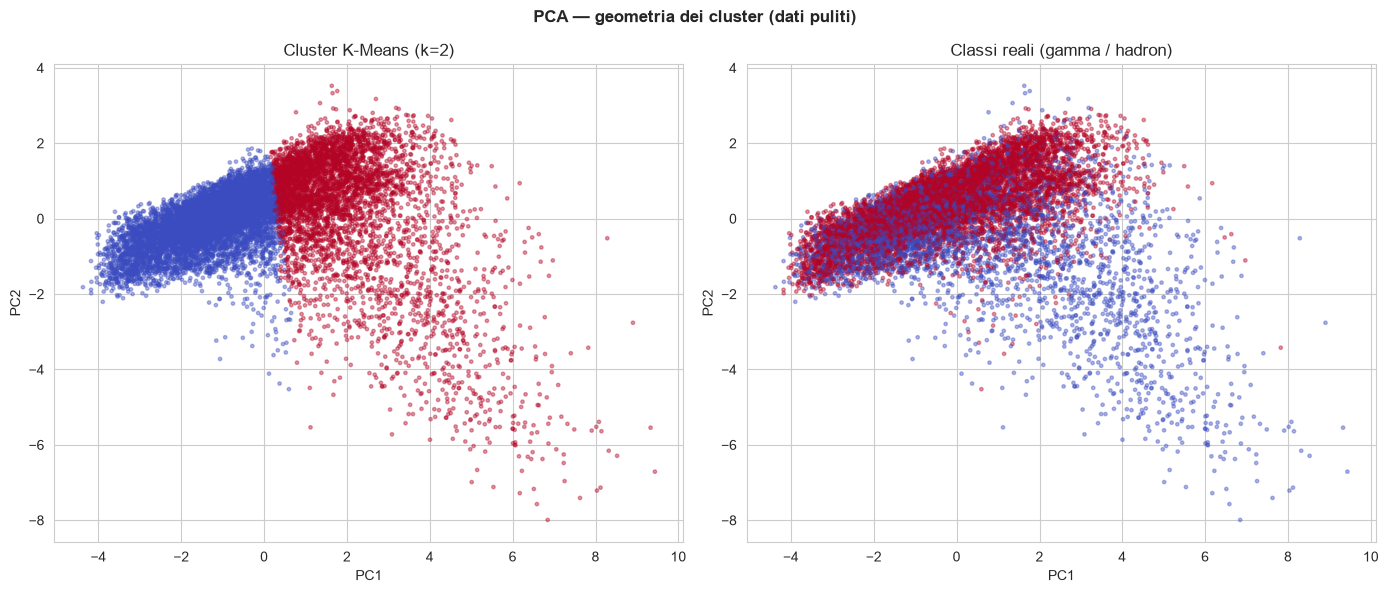
\includegraphics[width=0.98\textwidth]{kmeans_pca}
\caption{Proiezione PCA: i cluster geometrici non si allineano con la natura fisica e asimmetrica delle collisioni (ARI $\approx 0$).}
\label{fig:kmeans}
\end{figure}

Intromettendo crescenti interferenze nel flusso dei parametri originari 
(Figura~\ref{fig:kmeans_noise} e Figura~\ref{fig:kmeans_noise_pca}), 
l'evanescenza qualitativa subisce un drastico rialzo proporzionale. Mentre 
l'alterazione del labeling transita invisibile mantenendo gli scarti in 
stallo, le dispersioni standard espandono caoticamente le nuvole proiettate: 
le sagome dei grappoli si liquefanno in transizioni piatte causando riduzioni 
crescenti della compattezza (la silhouette cede fin oltre il traguardo dello $0{,}10$). 
La resilienza o vulnerabilità predittiva ad un determinato stress test è indissolubilmente legata 
al flusso dei vettori attivi immessi all'interno delle iterazioni prescelte dal 
progettista.

\begin{figure}[H]\centering
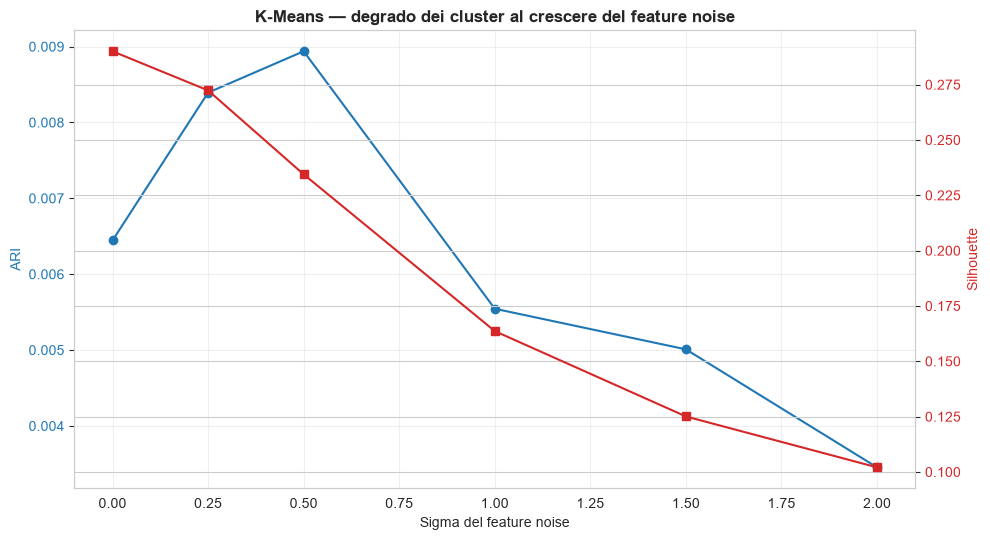
\includegraphics[width=0.86\textwidth]{kmeans_noise}
\caption{K-Means sotto feature noise: ARI e silhouette dei cluster. La silhouette cala, mentre l'ARI resta vicino a zero.}
\label{fig:kmeans_noise}
\end{figure}

\begin{figure}[H]\centering
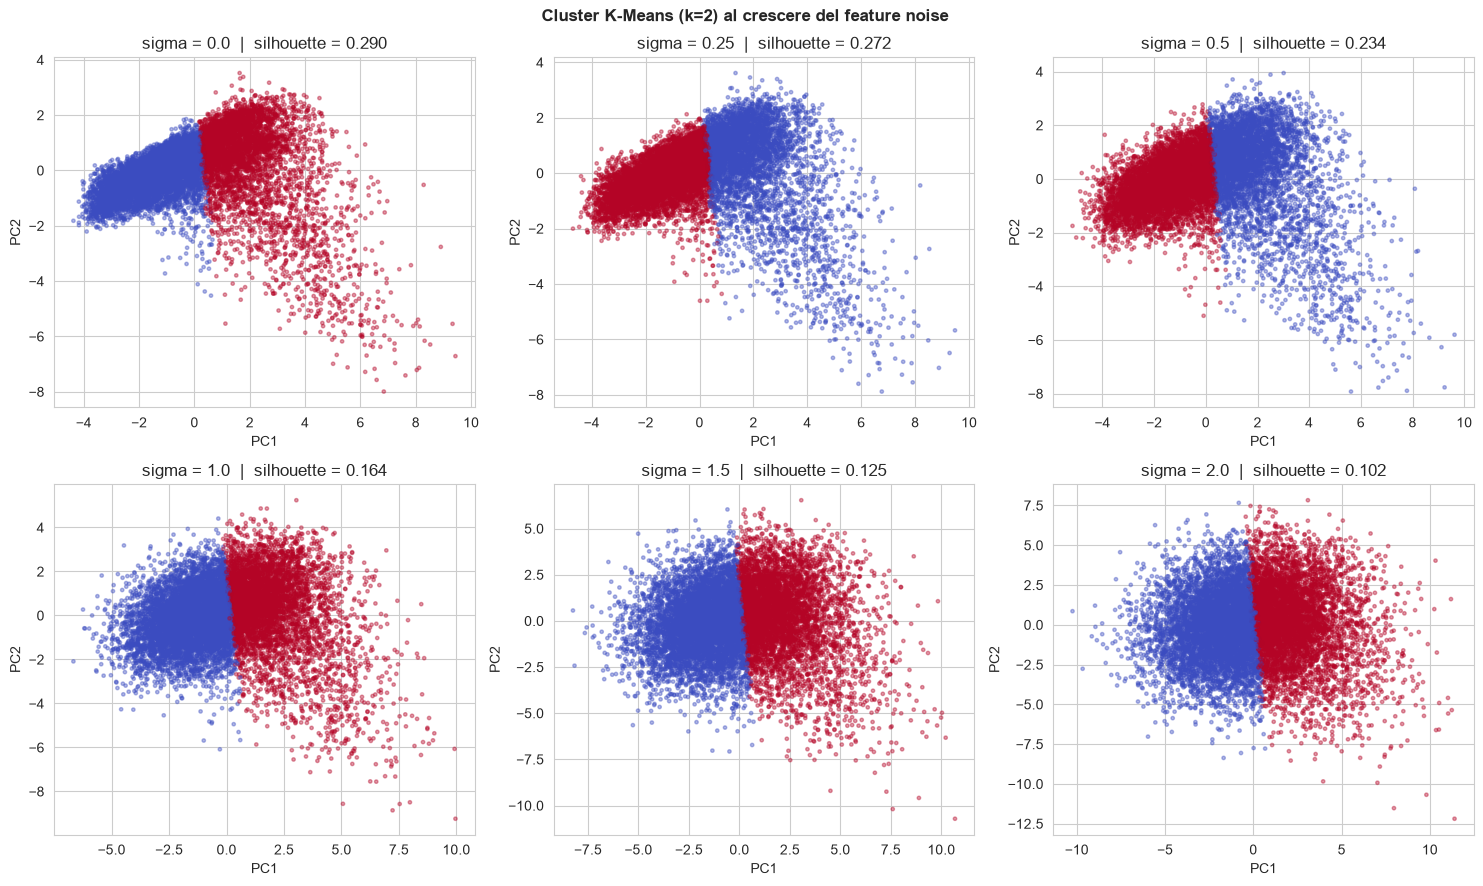
\includegraphics[width=0.92\textwidth]{kmeans_noise_pca}
\caption{Cluster K-Means (k=2) proiettati sulle prime due componenti (PCA). Al crescere del rumore ($\sigma$) la densità spaziale viene a mancare e le istanze sfumano i propri confini.}
\label{fig:kmeans_noise_pca}
\end{figure}

% ============================================================
% 12. CONCLUSIONI
% ============================================================
\section{Conclusioni}\label{sec:conclusioni}

Questo studio sposta l'attenzione dalla ricerca del modello migliore in assoluto
alla valutazione di quale algoritmo resista meglio a specifiche tipologie di 
corruzione dei dati. I risultati delineano un quadro coerente, in cui nessuna 
soluzione è priva di compromessi.

Tra i disturbi analizzati emerge una chiara gerarchia di pericolosità. Gli 
outlier risultano i meno dannosi, poiché il loro impatto è quasi trascurabile 
anche con trattamenti minimi. Feature noise e valori mancanti generano un calo 
prestazionale moderato e gestibile, mitigato rispettivamente dalla ridondanza 
informativa tra le feature e dalle strategie di imputazione. Al contrario, 
la rimozione delle feature e il label noise si rivelano le anomalie più critiche, 
seppur per ragioni opposte. La rimozione di una feature elimina informazione 
predittiva insostituibile: l'azzeramento della sola \texttt{fAlpha} risulta più 
impattante del livello massimo di feature noise. Il label noise, invece, forza 
le reti a memorizzare pattern errati. Il caso più estremo è rappresentato dal 
label noise borderline, che corrompe le istanze prossime al confine decisionale 
e riduce le prestazioni dei modelli a valori prossimi a quelli di un 
classificatore basato sulla classe maggioritaria.

Confrontando i modelli, nessuno prevale in ogni scenario. La rete Pro dimostra 
l'efficacia della regolarizzazione: l'\textit{early stopping} la rende 
particolarmente resistente al label noise random, bloccando la memorizzazione 
del rumore che penalizza la rete Base. Tuttavia, questa stessa propensione a 
non adattarsi troppo ai dati la penalizza leggermente quando una feature viene 
a mancare del tutto. Il Random Forest si conferma l'algoritmo più solido sui 
dati puliti, sui valori mancanti e sugli outlier, ma rivela una notevole fragilità 
di fronte all'inversione casuale delle etichette. La rete Base, pur essendo 
competitiva sui dati puliti, risulta la più esposta all'aumentare del rumore. 
La scelta del modello, pertanto, non può prescindere da un'analisi a priori 
sulle tipologie di errore attese nel dominio applicativo reale.

L'analisi separata per classe aggiunge un'ulteriore chiave di lettura. Sotto 
la maggior parte dei disturbi, il degrado non colpisce le classi in modo 
simmetrico: a peggiorare è quasi esclusivamente il riconoscimento della classe 
minoritaria (adroni), mentre il segnale (gamma) continua a essere identificato 
correttamente. L'utilizzo della sola accuratezza globale avrebbe mascherato 
questa dinamica. Per questo motivo, l'impiego dei \textit{class weight} nella 
rete Pro si rivela fondamentale per preservare la capacità di individuare la 
classe rara. Fa eccezione il label noise borderline, che degrada le metriche 
in modo uniforme su entrambe le classi poiché ne distorce direttamente il 
confine spaziale, vanificando il ribilanciamento.

L'evidenza più significativa riguarda tuttavia l'importanza del preprocessing 
rispetto alla complessità algoritmica. Strategie mirate, come l'imputazione
dei valori mancanti, la winsorizzazione degli outlier e l'interruzione 
dell'addestramento basata sulla validation loss, permettono di arginare gran 
parte del degrado prestazionale. Nessun modello, per quanto sofisticato, può 
recuperare un'informazione definitivamente cancellata o logicamente falsificata 
nei punti più sensibili. La robustezza di un sistema predittivo si costruisce 
a monte, nella cura del dato, tanto quanto a valle nella scelta dell'algoritmo. 
L'esperimento non supervisionato lo conferma ulteriormente: la vulnerabilità a 
uno specifico rumore dipende strettamente dalle informazioni che il modello 
sfrutta; ciò che risulta critico per un task supervisionato può rivelarsi 
del tutto ininfluente per un approccio basato puramente sulla distanza spaziale.

\end{document}